\pdfminorversion=4 % for acroread
%\documentclass[aspectratio=169,t,xcolor={usenames,dvipsnames}]{beamer}
\documentclass[aspectratio=169,t,handout,xcolor={usenames,dvipsnames}]{beamer}
\usepackage{../beamerstyle}
\usepackage{dsfont}
\usepackage{bm}
\usepackage[english]{babel}
\usepackage[utf8]{inputenc}
\usepackage{graphicx}
\usepackage{algorithm}
\usepackage[ruled,vlined,algo2e,linesnumbered]{algorithm2e}
%\usepackage[boxed,vlined]{algorithm2e}
\usepackage{hyperref}
\usepackage{booktabs}
\usepackage{mathtools}

\usepackage{amsmath,amssymb}
\usepackage{listings}
\lstset{frame=lines,framesep=3pt,numbers=left,numberblanklines=false,basicstyle=\ttfamily\small}

\usepackage{subfig}
\usepackage{multicol}
%\usepackage{appendixnumberbeamer}
%
\usepackage{tcolorbox}

\usepackage{pgfplots}
\usepackage{tikz}
\usetikzlibrary{trees} 
\usetikzlibrary{shapes.geometric}
\usetikzlibrary{positioning,shapes,shadows,arrows,calc,mindmap}
\usetikzlibrary{positioning,fadings,through}
\usetikzlibrary{decorations.pathreplacing}
\usetikzlibrary{intersections}
\usetikzlibrary{positioning,fit,calc,shadows,backgrounds}
\pgfdeclarelayer{background}
\pgfdeclarelayer{foreground}
\pgfsetlayers{background,main,foreground}
\tikzstyle{activity}=[rectangle, draw=black, rounded corners, text centered, text width=8em]
\tikzstyle{data}=[rectangle, draw=black, text centered, text width=8em]
\tikzstyle{myarrow}=[->, thick, draw=black]

% Define the layers to draw the diagram
\pgfdeclarelayer{background}
\pgfdeclarelayer{foreground}
\pgfsetlayers{background,main,foreground}

%\usepackage{listings}
%\lstset{numbers=left,
%  showstringspaces=false,
%  frame={tb},
%  captionpos=b,
%  lineskip=0pt,
%  basicstyle=\ttfamily,
%%  extendedchars=true,
%  stepnumber=1,
%  numberstyle=\small,
%  xleftmargin=1em,
%  breaklines
%}

 
\definecolor{blue}{RGB}{0, 74, 153}

\usetheme{Boadilla}
%\useinnertheme{rectangles}
\usecolortheme{whale}
\setbeamercolor{alerted text}{fg=blue}
\useoutertheme{infolines}
\setbeamertemplate{navigation symbols}{\vspace{-5pt}} % to lower the logo
\setbeamercolor{date in head/foot}{bg=white} % blue
\setbeamercolor{date in head/foot}{fg=white}
\setbeamercolor{author  in head/foot}{bg=white} %blue
\setbeamercolor{title in head/foot}{bg=white} % blue
\setbeamercolor{title}{fg=white, bg=blue}
\setbeamercolor{block title}{fg=white,bg=blue}
\setbeamercolor{block body}{bg=blue!10}
\setbeamercolor{frametitle}{fg=white, bg=blue}
\setbeamercovered{invisible}

\makeatletter
\setbeamertemplate{footline}
{
  \leavevmode%
  \hbox{%
  \begin{beamercolorbox}[wd=.333333\paperwidth,ht=2.25ex,dp=1ex,center]{author in head/foot}%
%    \usebeamerfont{author in head/foot}\insertshortauthor
  \end{beamercolorbox}%
  \begin{beamercolorbox}[wd=.333333\paperwidth,ht=2.25ex,dp=1ex,center]{title in head/foot}%
    \usebeamerfont{title in head/foot}\insertshorttitle
  \end{beamercolorbox}%
  \begin{beamercolorbox}[wd=.333333\paperwidth,ht=2.25ex,dp=1ex,right]{date in head/foot}%
    \usebeamerfont{date in head/foot}\insertshortdate{}\hspace*{2em}
%    \insertframenumber\hspace*{2ex} 
  \end{beamercolorbox}}%
  \vskip0pt%
}
\makeatother

%\pgfdeclareimage[height=1.2cm]{automl}{images/logos/automl.png}
%\pgfdeclareimage[height=1.2cm]{freiburg}{images/logos/freiburg}

%\logo{\pgfuseimage{freiburg}}

\renewcommand{\comment}[1]{
	\noindent
	%\vspace{0.25cm}
	{\color{red}{\textbf{TODO:} #1}}
	%\vspace{0.25cm}
}
\newcommand{\notefh}[1]{\textcolor{red}{\textbf{FH:} #1}}
\renewcommand{\comment}[1]{}
\newcommand{\hide}[1]{}
\newcommand{\cemph}[2]{\emph{\textcolor{#1}{#2}}}

\newcommand{\lit}[1]{{\footnotesize\color{black!60}[#1]}}

\newcommand{\litw}[1]{{\footnotesize\color{blue!20}[#1]}}


\newcommand{\myframe}[2]{\begin{frame}[c]{#1}#2\end{frame}}
\newcommand{\myframetop}[2]{\begin{frame}{#1}#2\end{frame}}
\newcommand{\myit}[1]{\begin{itemize}#1\end{itemize}}
\newcommand{\myblock}[2]{\begin{block}{#1}#2\end{block}}


\newcommand{\votepurple}[1]{\textcolor{Purple}{$\bigstar$}}
\newcommand{\voteyellow}[1]{\textcolor{Goldenrod}{$\bigstar$}}
\newcommand{\voteblue}[1]{\textcolor{RoyalBlue}{$\bigstar$}}
\newcommand{\votepink}[1]{\textcolor{Pink}{$\bigstar$}}

\newcommand{\diff}{\mathop{}\!\mathrm{d}}
\newcommand{\refstyle}[1]{{\small{\textcolor{gray}{#1}}}}
\newcommand{\hands}[0]{
\includegraphics[height=1.5em]{images/hands}}
\newcommand{\transpose}[0]{{\textrm{\tiny{\sf{T}}}}}
\newcommand{\norm}{{\mathcal{N}}}
\newcommand{\cutoff}[0]{\kappa}
\newcommand{\instD}[0]{\dataset}
\newcommand{\insts}[0]{\mathcal{I}}
\newcommand{\inst}[0]{i}
\newcommand{\instI}[1]{i^{(#1)}}

% Iteration specific instance of variable/function/anything
% Introduced in the BO section, but moved up here to make it available within other macros
\newcommand{\iter}[2][\bocount]{{#2}^{(#1)}}

%--------HPO parameter macros-----------

% Parameter Configuration Space
\newcommand{\pcs}[0]{\pmb{\Lambda}}

% ???
\newcommand{\bx}[0]{\conf}

% Parameter Configuration
\newcommand{\conf}[0]{\pmb{\lambda}}

% Final Configuration
\newcommand{\finconf}[0]{\pmb{\hat{\lambda}}}

% Configuration corresponding to a given iteration -- better use \iter!
\newcommand{\confI}[1]{{\conf}^{(#1)}}

% Default Configuration
\newcommand{\defconf}[0]{{\conf}_{\text{def}}}

% Incumbent Configuration
\newcommand{\incumbent}[1][\bocount]{\iter[#1]{\finconf}}

% Optimal Configuration
\newcommand{\optconf}[0]{{\conf}^*}

% Configuration Space
\newcommand{\confs}[0]{\pcs}

%----------------------------------------

%\newcommand{\vlambda}[0]{\bm{\lambda}}
%\newcommand{\vLambda}[0]{\bm{\Lambda}}
\newcommand{\dataset}[0]{\mathcal{D}}
\newcommand{\datasets}[0]{\mathbf{D}}
\newcommand{\loss}[0]{L}
\newcommand{\risk}{\mathcal{R}}
\newcommand{\riske}{\mathcal{R}_{\text{emp}}}
\newcommand{\cost}[0]{c}
\newcommand{\costI}[1]{c^{(#1)}}

% Gaussian Process
\newcommand{\gp}{\mathcal{G}}
% Family of Objective Functions
\newcommand{\objF}{F}

%---------------BO Macros------------------

% BO loop counter
\newcommand{\bocount}{t}
% BO loop counter max, the counter runs from 1 to this value
\newcommand{\bobudget}{T}
% BO loop observation
\newcommand{\obs}[1][\conf]{\cost({#1})}
% BO loop observation space
\newcommand{\obsspace}{\mathcal{Y}}
% BO loop next observation
\newcommand{\bonextobs}{\obs[\iter{\conf}]}
% Acquisition Function, no args
\newcommand{\acq}{u}
% Standard Normal PDF
\newcommand{\pdf}{\phi}
% Standard Normal CDF
\newcommand{\cdf}{\Phi}
% Mean
\newcommand{\mean}{\mu}
% Standard Deviation
\newcommand{\stddev}{\sigma}
% Variance
\newcommand{\variance}{\sigma^2}
% Noise
\newcommand{\noise}{\nu}
% BO loop next selected sample
\newcommand{\bonextsample}{\confI{\bocount}}

% Single hyperparameter
\newcommand{\hyperparam}{\lambda}

% Single hyperparameter within a hyperparameter configuration
\newcommand{\hyperparami}[1][i]{{\hyperparam}_#1}

% Full definition of final configuration
\newcommand{\finconffull}{\incumbent[\bobudget]}

% Dataset
\newcommand{\datasetHPO}{{\dataset}_{HPO}}

% Dataset definition
\newcommand{\datasetHPOdef}{{\langle \bonextsample,\,\bonextobs \rangle}_{\bocount=1}^{\bobudget}}

% Double Display Fraction, forces large displays for everything in numerator and denominator
\newcommand\ddfrac[2]{\frac{\displaystyle #1}{\displaystyle #2}}

% Conditional Probability "Given That" Relation, source:https://tex.stackexchange.com/a/141685/205886
\newcommand\given[1][]{\:#1\vert\:}

% Expectation as a math operator
\DeclareMathOperator*{\E}{\mathbb{E}}

% Citation 
\newcommand{\source}[1]{
    \begin{flushright}
    	Source: \lit{#1}
    \end{flushright}
}
%-------------------------------------------

%Real numbers set
\newcommand{\realnum}{\mathbb{R}}
%Configuration space - do not use
%\newcommand{\configspace}{\Theta}
%Instances - do not use
%\newcommand{\instances}{\mathcal{I}}
%Expected value
\newcommand{\expectation}{\mathbb{E}}
%Kernel
\newcommand{\kernel}{\kappa}
%Constraint function
\newcommand{\constraintf}{c}
%Normal distribution
\newcommand{\normaldist}{\mathcal{N}}

% \renewcommand{\vec}[1]{\mathbf{#1}}
\newcommand{\hist}[0]{\dataset_{\text{Hist}}}
\newcommand{\param}[0]{p}
\newcommand{\algo}[0]{\mathcal{A}}
\newcommand{\algos}[0]{\mathbf{A}}
%\newcommand{\nn}[0]{N}
\newcommand{\feats}[0]{\mathcal{X}_{\text{meta}}}
\newcommand{\feat}[0]{\x_{\text{meta}}}
%\newcommand{\cluster}[0]{\vec{h}}
%\newcommand{\clusters}[0]{\vec{H}}
\newcommand{\perf}[0]{\mathbb{R}}
%\newcommand{\surro}[0]{\mathcal{S}}
\newcommand{\surro}[0]{\hat{\cost}}
\newcommand{\func}[0]{f}
\newcommand{\epm}[0]{\surro}
\newcommand{\portfolio}[0]{\mathbf{P}}
\newcommand{\schedule}[0]{\mathcal{S}}

% Machine Learning
\newcommand{\mdata}[0]{\dataset_{\text{meta}}}
\newcommand{\datasettrain}[0]{\dataset_{\text{train}}}
\newcommand{\datasetval}[0]{\dataset_{\text{val}}}
\newcommand{\datasettest}[0]{\dataset_{\text{test}}}
\newcommand{\x}[0]{\mathbf{x}}
\newcommand{\y}[0]{y}
\newcommand{\xI}[1]{\mathbf{x}^{(#1)}}
\newcommand{\yI}[1]{y^{(#1)}}
\newcommand{\fx}{f(\mathbf{x})}  % f(x), continuous prediction function
\newcommand{\Hspace}{\mathcal{H}} % hypothesis space where f is from
\newcommand{\fh}{\hat{f}}       % f hat, estimated prediction function

% Deep Learning
\newcommand{\weights}[0]{\theta}
\newcommand{\metaweights}[0]{\phi}


% reinforcement learning
\newcommand{\policies}[0]{\mathbf{\Pi}}
\newcommand{\policy}[0]{\pi}
\newcommand{\actionRL}[0]{a}
\newcommand{\stateRL}[0]{s}
\newcommand{\statesRL}[0]{\mathcal{S}}
\newcommand{\rewardRL}[0]{r}
\newcommand{\rewardfuncRL}[0]{\mathcal{R}}

\RestyleAlgo{algoruled}
\DontPrintSemicolon
\LinesNumbered
\SetAlgoVlined
\SetFuncSty{textsc}

\SetKwInOut{Input}{Input}
\SetKwInOut{Output}{Output}
\SetKw{Return}{return}

%\newcommand{\changed}[1]{{\color{red}#1}}

%\newcommand{\citeN}[1]{\citeauthor{#1}~(\citeyear{#1})}

\renewcommand{\vec}[1]{\mathbf{#1}}
\DeclareMathOperator*{\argmin}{arg\,min}
\DeclareMathOperator*{\argmax}{arg\,max}

%\newcommand{\aqme}{\textit{AQME}}
%\newcommand{\aslib}{\textit{ASlib}}
%\newcommand{\llama}{\textit{LLAMA}}
%\newcommand{\satzilla}{\textit{SATzilla}}
%\newcommand{\satzillaY}[1]{\textit{SATzilla'{#1}}}
%\newcommand{\snnap}{\textit{SNNAP}}
%\newcommand{\claspfolioTwo}{\textit{claspfolio~2}}
%\newcommand{\flexfolio}{\textit{FlexFolio}}
%\newcommand{\claspfolioOne}{\textit{claspfolio~1}}
%\newcommand{\isac}{\textit{ISAC}}
%\newcommand{\eisac}{\textit{EISAC}}
%\newcommand{\sss}{\textit{3S}}
%\newcommand{\sunny}{\textit{Sunny}}
%\newcommand{\ssspar}{\textit{3Spar}}
%\newcommand{\cshc}{\textit{CSHC}}
%\newcommand{\cshcpar}{\textit{CSHCpar}}
%\newcommand{\measp}{\textit{ME-ASP}}
%\newcommand{\aspeed}{\textit{aspeed}}
%\newcommand{\autofolio}{\textit{AutoFolio}}
%\newcommand{\cedalion}{\textit{Cedalion}}
\newcommand{\fanova}{\textit{fANOVA}}
\newcommand{\sbs}{\textit{SB}}
\newcommand{\oracle}{\textit{VBS}}

% like approaches
\newcommand{\claspfoliolike}[1]{\texttt{claspfolio-#1-like}}
\newcommand{\satzillalike}[1]{\texttt{SATzilla'#1-like}}
\newcommand{\isaclike}{\texttt{ISAC-like}}
\newcommand{\ssslike}{\texttt{3S-like}}
\newcommand{\measplike}{\texttt{ME-ASP-like}}

\newcommand{\irace}{\textit{I/F-race}}
\newcommand{\gga}{\textit{GGA}}
\newcommand{\smac}{\textit{SMAC}}
\newcommand{\paramils}{\textit{ParamILS}}
\newcommand{\spearmint}{\textit{Spearmint}}
\newcommand{\tpe}{\textit{TPE}}


\usepackage{pifont}
\newcommand{\itarrow}{\mbox{\Pisymbol{pzd}{229}}}
\newcommand{\ithook}{\mbox{\Pisymbol{pzd}{52}}}
\newcommand{\itcross}{\mbox{\Pisymbol{pzd}{56}}}
\newcommand{\ithand}{\mbox{\raisebox{-1pt}{\Pisymbol{pzd}{43}}}}

%\DeclareMathOperator*{\argmax}{arg\,max}

\newcommand{\ie}{{\it{}i.e.\/}}
\newcommand{\eg}{{\it{}e.g.\/}}
\newcommand{\cf}{{\it{}cf.\/}}
\newcommand{\wrt}{\mbox{w.r.t.}}
\newcommand{\vs}{{\it{}vs\/}}
\newcommand{\vsp}{{\it{}vs\/}}
\newcommand{\etc}{{\copyedit{etc.}}}
\newcommand{\etal}{{\it{}et al.\/}}

\newcommand{\pscProc}{{\bf procedure}}
\newcommand{\pscBegin}{{\bf begin}}
\newcommand{\pscEnd}{{\bf end}}
\newcommand{\pscEndIf}{{\bf endif}}
\newcommand{\pscFor}{{\bf for}}
\newcommand{\pscEach}{{\bf each}}
\newcommand{\pscThen}{{\bf then}}
\newcommand{\pscElse}{{\bf else}}
\newcommand{\pscWhile}{{\bf while}}
\newcommand{\pscIf}{{\bf if}}
\newcommand{\pscRepeat}{{\bf repeat}}
\newcommand{\pscUntil}{{\bf until}}
\newcommand{\pscWithProb}{{\bf with probability}}
\newcommand{\pscOtherwise}{{\bf otherwise}}
\newcommand{\pscDo}{{\bf do}}
\newcommand{\pscTo}{{\bf to}}
\newcommand{\pscOr}{{\bf or}}
\newcommand{\pscAnd}{{\bf and}}
\newcommand{\pscNot}{{\bf not}}
\newcommand{\pscFalse}{{\bf false}}
\newcommand{\pscEachElOf}{{\bf each element of}}
\newcommand{\pscReturn}{{\bf return}}

%\newcommand{\param}[1]{{\sl{}#1}}
\newcommand{\var}[1]{{\it{}#1}}
\newcommand{\cond}[1]{{\sf{}#1}}
%\newcommand{\state}[1]{{\sf{}#1}}
%\newcommand{\func}[1]{{\sl{}#1}}
\newcommand{\set}[1]{{\Bbb #1}}
%\newcommand{\inst}[1]{{\tt{}#1}}
\newcommand{\myurl}[1]{{\small\sf #1}}

\newcommand{\Nats}{{\Bbb N}}
\newcommand{\Reals}{{\Bbb R}}
\newcommand{\extset}[2]{\{#1 \; | \; #2\}}

\newcommand{\vbar}{$\,\;|$\hspace*{-1em}\raisebox{-0.3mm}{$\,\;\;|$}}
\newcommand{\vendbar}{\raisebox{+0.4mm}{$\,\;|$}}
\newcommand{\vend}{$\,\:\lfloor$}


\newcommand{\goleft}[2][.7]{\parbox[t]{#1\linewidth}{\strut\raggedright #2\strut}}
\newcommand{\rightimage}[2][.3]{\mbox{}\hfill\raisebox{1em-\height}[0pt][0pt]{\includegraphics[width=#1\linewidth]{#2}}\vspace*{-\baselineskip}}






\title{AutoML: Bayesian Optimization for HPO}
\subtitle{Overview of Bayesian Optimization}
\author[Marius Lindauer]{Bernd Bischl \and \underline{Frank Hutter} \and Lars Kotthoff\newline \and Marius Lindauer \and Joaquin Vanschoren}
\institute{}
\date{}
    
    
    
\begin{document}
\maketitle
   
%-----------------------------------------------------------------------
\begin{frame}[c]{Global Blackbox Optimization}
    
    \begin{itemize}
        \item Consider the \alert{global optimization problem} of finding: 
        \[\conf^* \in \argmin_{\conf \in \confs} f(\conf)\]
        
\pause
        \item In the most general form, function $f$ is a \alert{blackbox function}:
    	
    	\begin{center}
\scalebox{0.5}{\newcommand{\myblackbox}{\fcolorbox{black}{black}{
    \minipage[t]{\dimexpr0.111\linewidth-2\fboxsep-2\fboxrule\relax}
        ~~~\\
        ~~~\\
        ~~~\\
    \endminipage}}
    
    
    	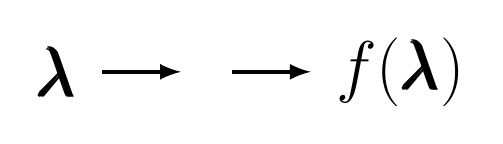
\begin{tikzpicture}
\tikzstyle{every node}=[draw,fill=white,minimum width=0cm,thin]
\tikzstyle{every path}=[-latex,ultra thick]
\node (A) [draw=white]{{\Huge{$\conf$}}};
\node (B) [right=14mm of A,draw=white] {\myblackbox{}};
\node (C) [right=14mm of B,draw=white] {{\Huge{$f(\conf)$}}};
%\node (D) [below=7mm of B, align=center, fill=black!10] {\large{Bayesian}\\\large{optimization}};

\draw ($(A.east)+(0.2,0.0)$) -- ($(B.west)+(-0.2,0.0)$);
\draw ($(B.east)+(0.2,0.0)$) -- ($(C.west)+(-0.2,0.0)$);
%\draw ($(C.south)+(0.0,-0.2)$) -| ++(0.0,0.0) |- ($(D.east)+(0.2,0.0)$);
%\draw ($(D.west)+(-0.2,0.0)$) |- ++(0.0,0.0) -| ($(A.south)+(0.0,-0.2)$);
\end{tikzpicture}
}
    	\end{center}

   %\end{itemize}
    
   \begin{itemize}
    	\item Only mode of interaction with $f$: querying $f$'s value at a given $\conf$ 
        \item Function $f$ may not be available in closed form, not convex, not differentiable, noisy, etc. 
   \end{itemize}
    	%}   
\medskip
\pause

        \item Today, we'll discuss a \alert{Bayesian} approach for solving such blackbox optimization problems
\medskip
\pause
        \item Blackbox optimization can be used for hyperparameter optimization (HPO)
    %\end{itemize}
   	 	\begin{itemize}
         	\item Define \alert{$f(\conf) := \mathcal{L}( \mathcal{A}_{\conf}, \mathcal{D}_{train}, \mathcal{D}_{valid} )$}
        	\item Note: for formulations of HPO that go beyond blackbox optimization, see next lecture
        \end{itemize}
    \end{itemize}    
\end{frame}

%----------------------------------------------------------------------
%\begin{frame}[c]{Optimization problem example}

%We know that:
%\begin{itemize}
%    \item The function $\cost$ is Lipschitz continuous and differentiable.
%    \fhpause
%    \item The minimizer of $\cost$ is in the interval [0,1].
%    \fhpause
%    \item We have observed 3 evaluations of $\cost$.
%\end{itemize}

%\end{frame}
%----------------------------------------------------------------------
%\begin{frame}[c]{Problem description}
%\framesubtitle{We have 4 function evaluations}
%\begin{figure}
%    \centering
%    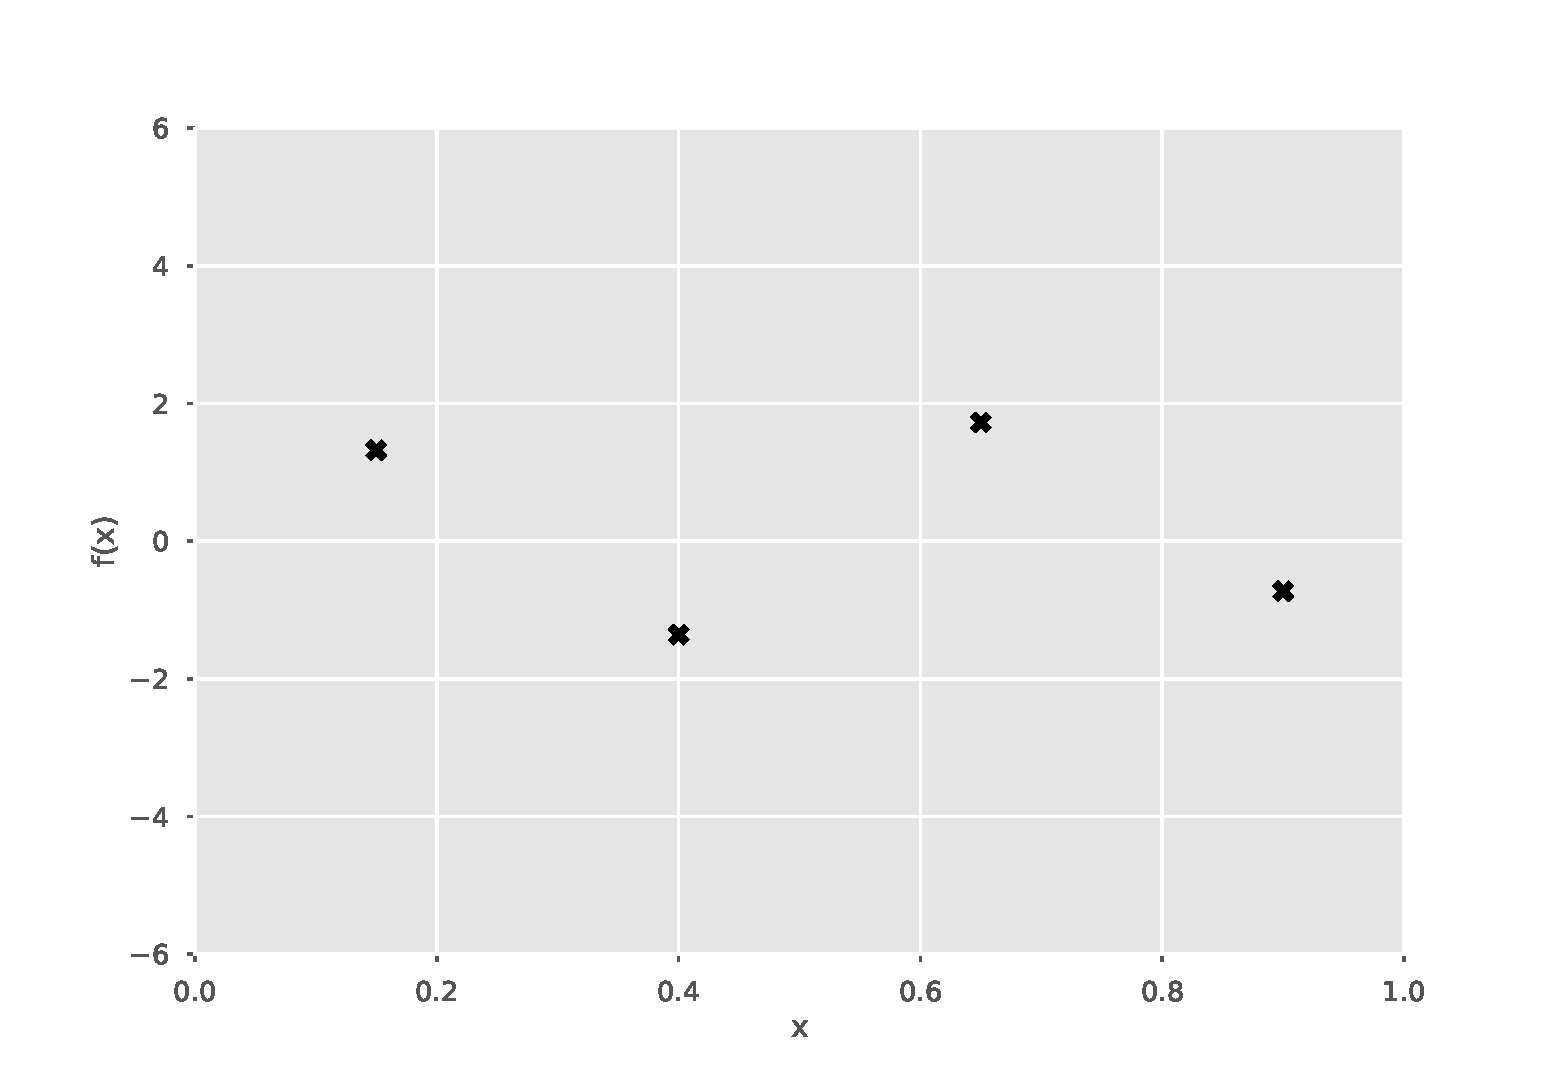
\includegraphics[width=0.8\textwidth, %height=0.38\textwidth]{images/intro_images/plot_datapoints.p%df}
%    \label{fig:my_label}
%\end{figure}
%\begin{center}
%  Where is the minimum of function $f$?  
%\end{center}
%\source{Plots are based on Javier Gonz\'alez's BO lecture %(bo\_intro.py)}



%\end{frame}

%-----------------------------------------------------------------------
%----------------------------------------------------------------------
%\begin{frame}[c]{Problem description}
%\framesubtitle{One possible curve}
%\begin{figure}
%    \centering
%    \includegraphics[width=0.7\textwidth, %height=0.4\textwidth]{images/intro_images/plot_posterior_1_s%ample.pdf}
%    \label{fig:my_label}
%\end{figure}
%\source{Plots are based on Javier Gonz\'alez's BO lecture %(bo\_intro.py)}



%\end{frame}

%-----------------------------------------------------------------------
%----------------------------------------------------------------------
%\begin{frame}[c]{Problem description}
%\framesubtitle{Three possible curves}
%\begin{figure}
%    \centering
%    \includegraphics[width=0.7\textwidth, %height=0.4\textwidth]{images/intro_images/plot_posterior_3_s%ample.pdf}
%    \label{fig:my_label}
%\end{figure}
%\source{Plots are based on Javier Gonz\'alez's BO lecture %(bo\_intro.py)}



%\end{frame}

%-----------------------------------------------------------------------
%----------------------------------------------------------------------
%\begin{frame}[c]{Problem description}
%\framesubtitle{Ten possible curves}
%\begin{figure}
%    \centering
%    \includegraphics[width=0.7\textwidth, %height=0.4\textwidth]{images/intro_images/plot_posterior_10_%sample.pdf}
%    \label{fig:my_label}
%\end{figure}
%\source{Plots are based on Javier Gonz\'alez's BO lecture %(bo\_intro.py)}



%\end{frame}

%-----------------------------------------------------------------------
%----------------------------------------------------------------------
%\begin{frame}[c]{Problem description}
%\framesubtitle{One hundred possible curves}
%\begin{figure}
%    \centering
%    \includegraphics[width=0.7\textwidth, %height=0.4\textwidth]{images/intro_images/plot_posterior_100%_sample.pdf}
%    \label{fig:my_label}
%\end{figure}
%\source{Plots are based on Javier Gonz\'alez's BO lecture %(bo\_intro.py)}



%\end{frame}

%-----------------------------------------------------------------------%----------------------------------------------------------------------
%\begin{frame}[c]{Problem description}
%\framesubtitle{One thousand possible curves}
%\begin{figure}
%    \centering
%    \includegraphics[width=0.7\textwidth, %height=0.4\textwidth]{images/intro_images/plot_posterior_100%0_sample.pdf}
%    \label{fig:my_label}
%\end{figure}
%\source{Plots are based on Javier Gonz\'alez's BO lecture (bo\_intro.py)}



%\end{frame}

%-----------------------------------------------------------------------
%----------------------------------------------------------------------
%\begin{frame}[c]{Problem description}
%\framesubtitle{Infinitely many curves}
%\begin{figure}
%    \centering
%    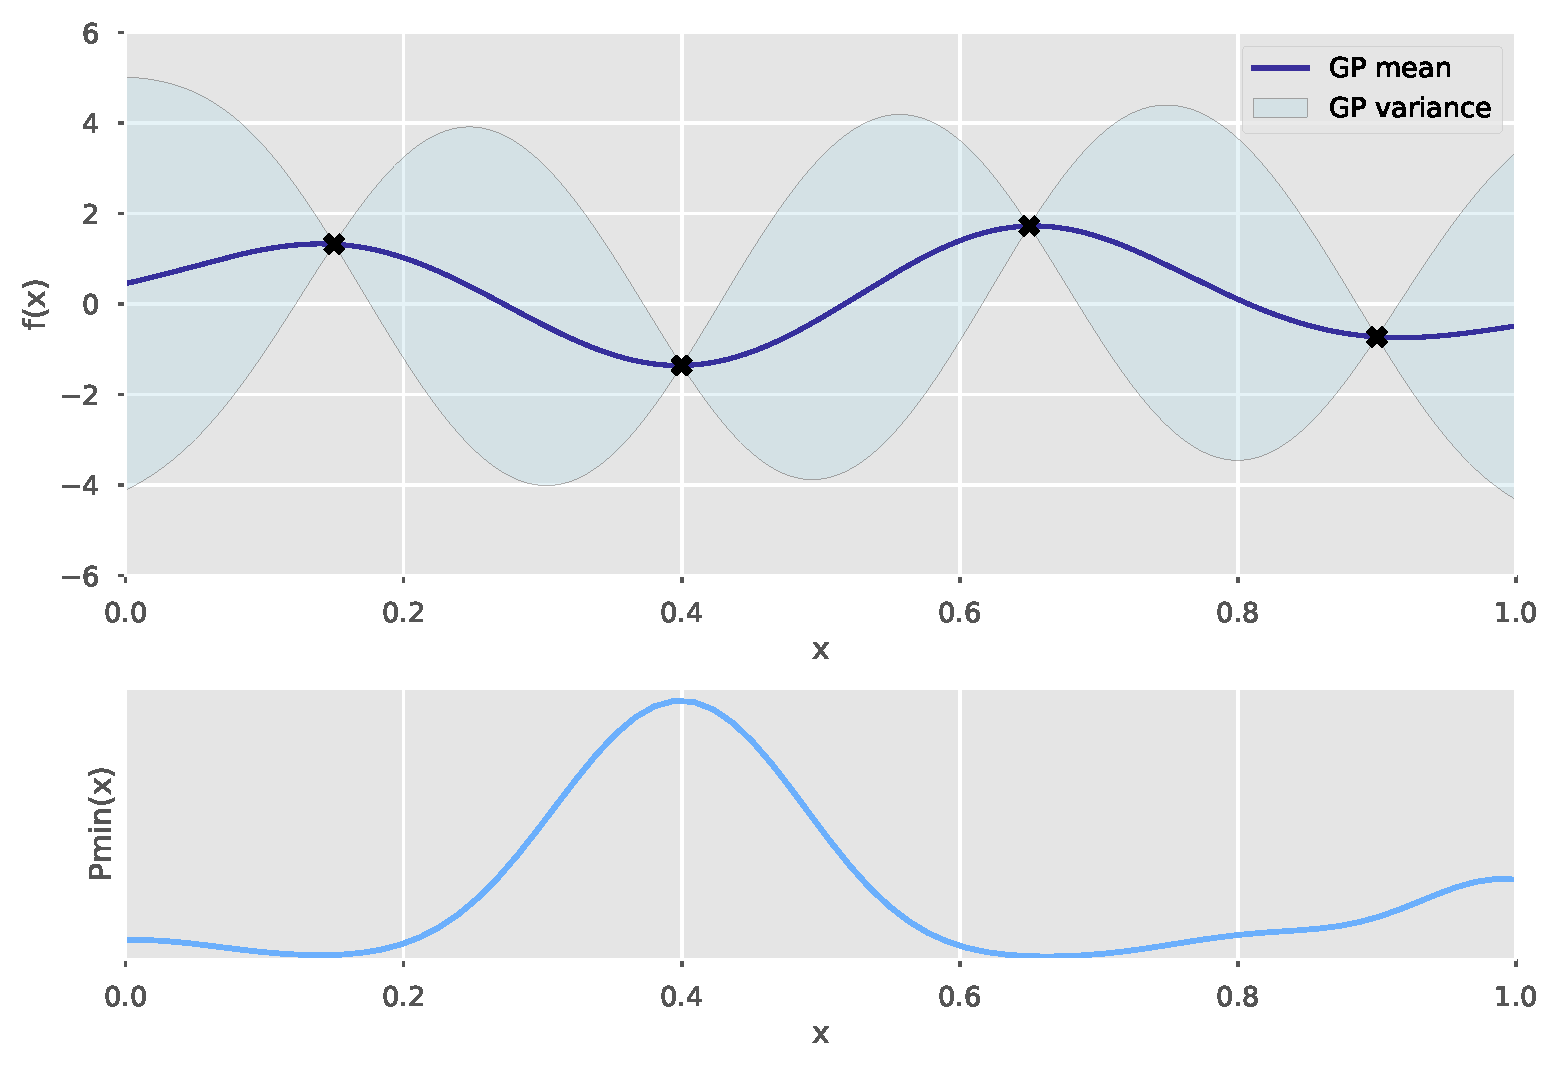
\includegraphics[width=0.7\textwidth, %height=0.4\textwidth]{images/intro_images/plot_posterior.pdf%}
%    \label{fig:my_label}
%\end{figure}
%\source{Plots are based on Javier Gonz\'alez's BO lecture (bo\_intro.py)}


%\end{frame}
%----------------------------------------------------------------------
\myframetop{Bayesian Optimization of a blackbox function in a nutshell}{

\bigskip
\bigskip
\bigskip

    \onslide<1->
    \begin{figure}
        \vspace{-1em}
        \centering
        \only<1>{
            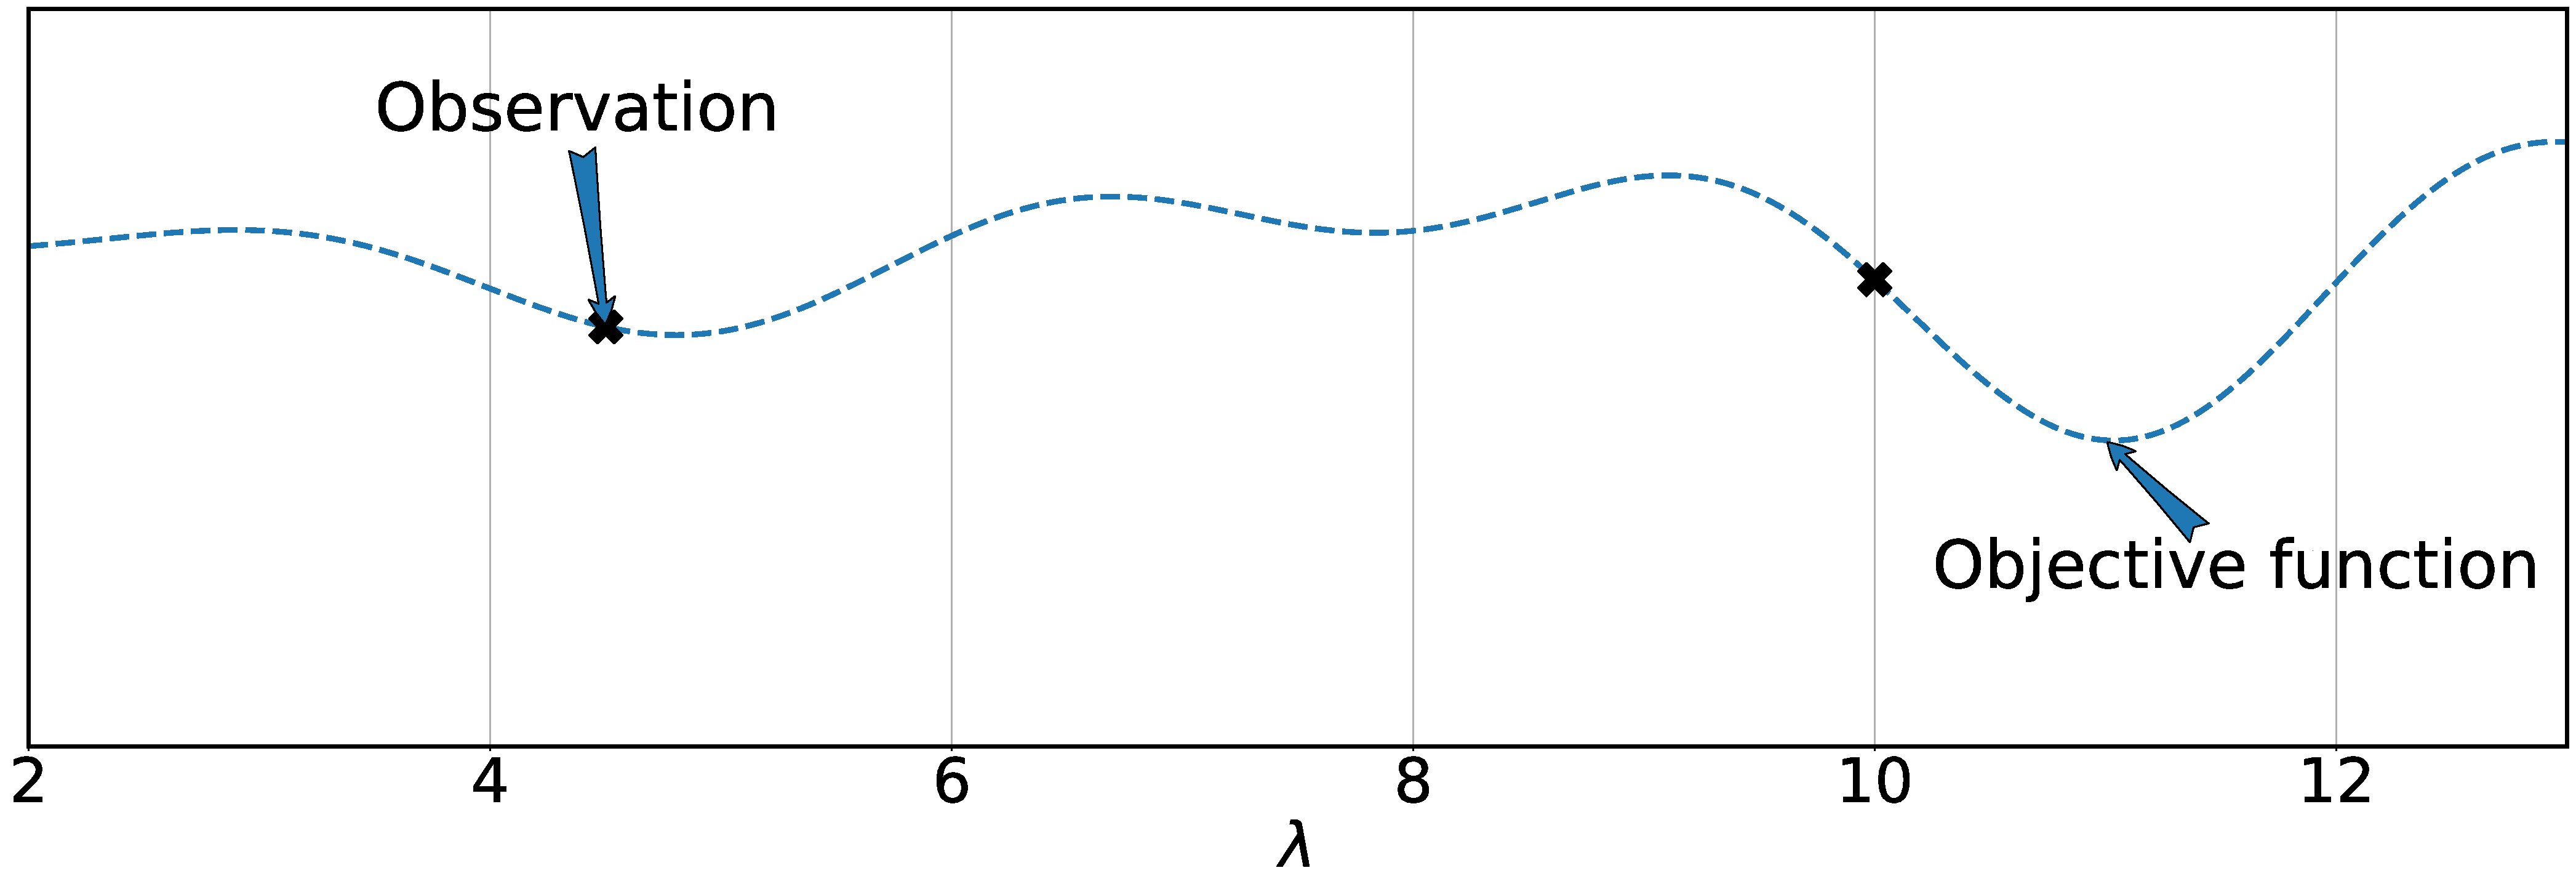
\includegraphics[width=0.95\textwidth]{images/intro_images/IntroPlots_Obs.pdf}
        }\only<2>{
            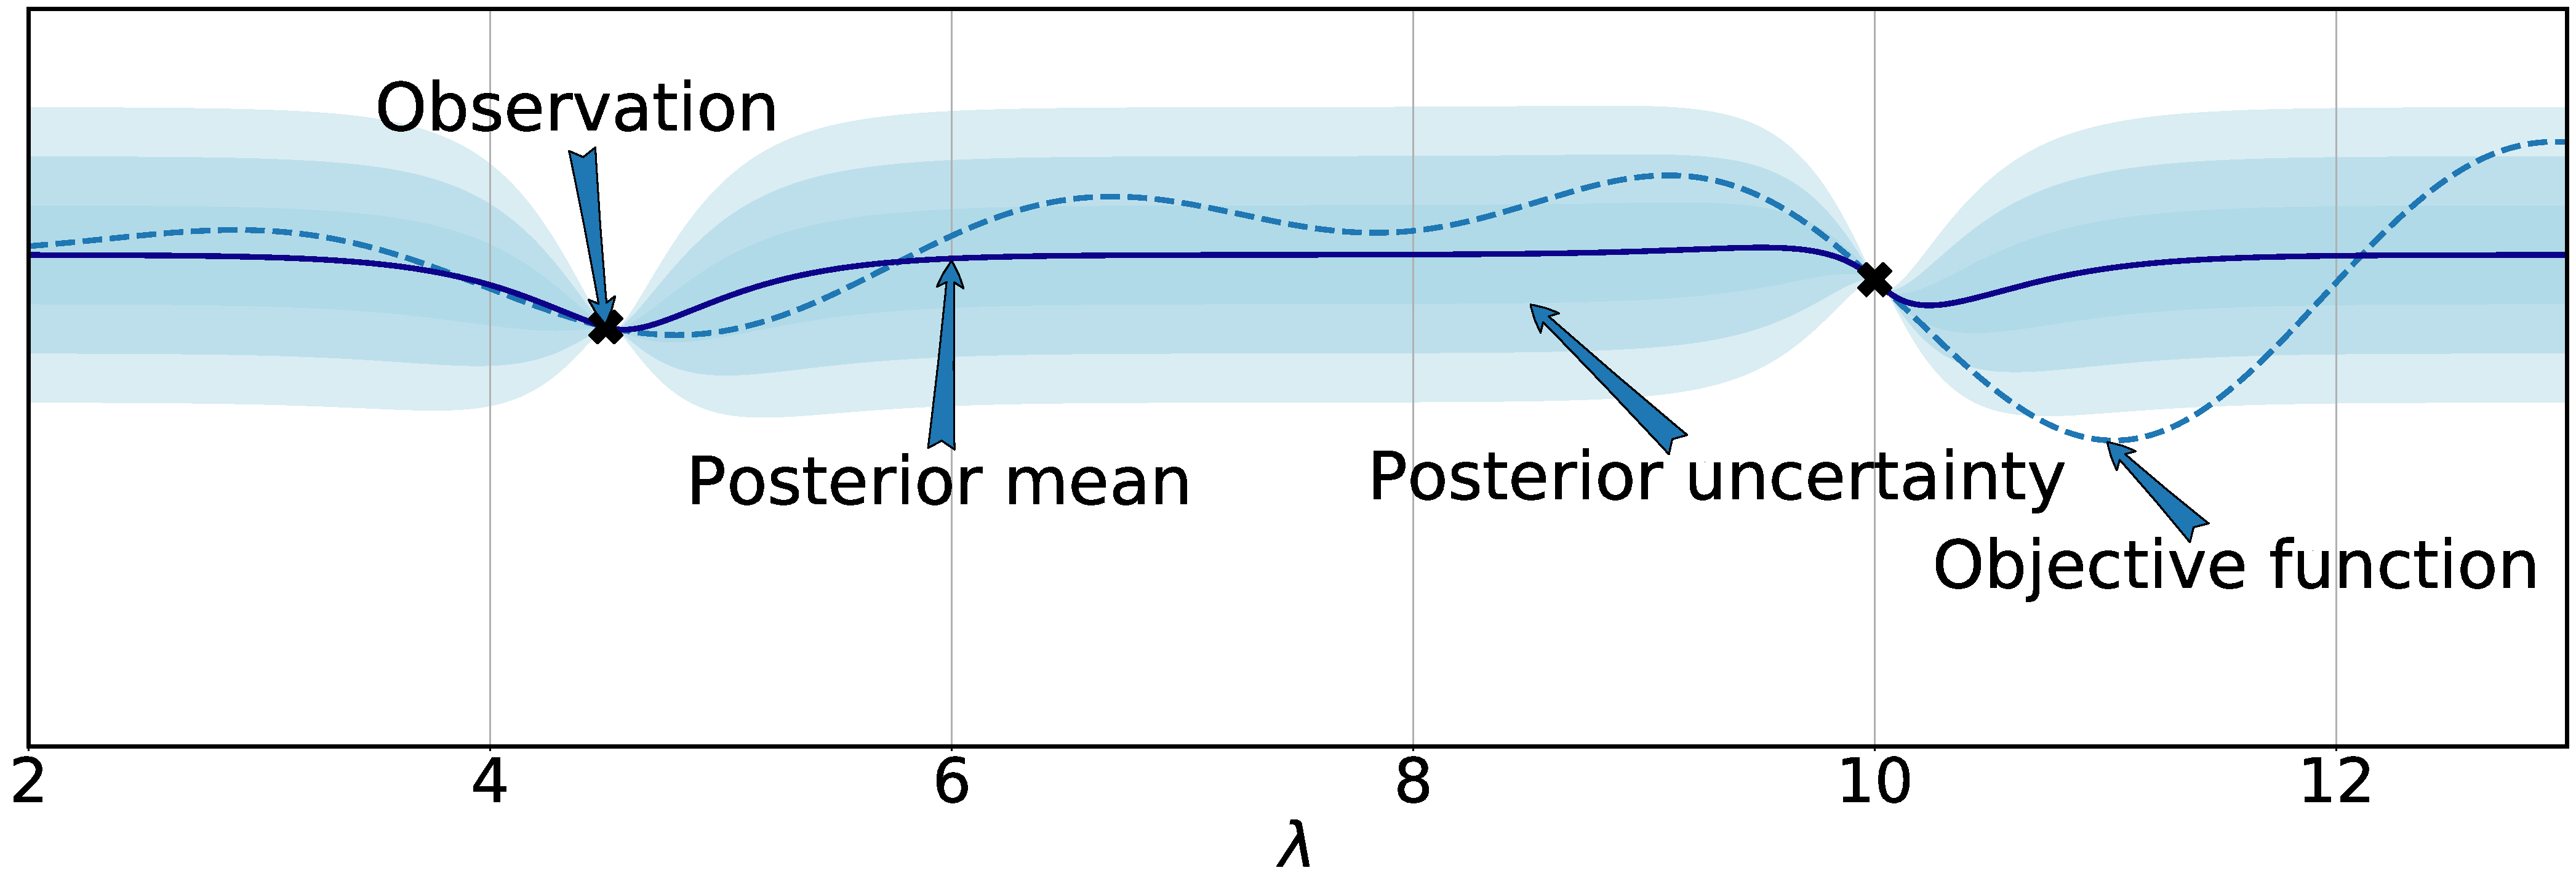
\includegraphics[width=0.95\textwidth]{images/intro_images/IntroPlots_GP.pdf}
        }\only<3>{
            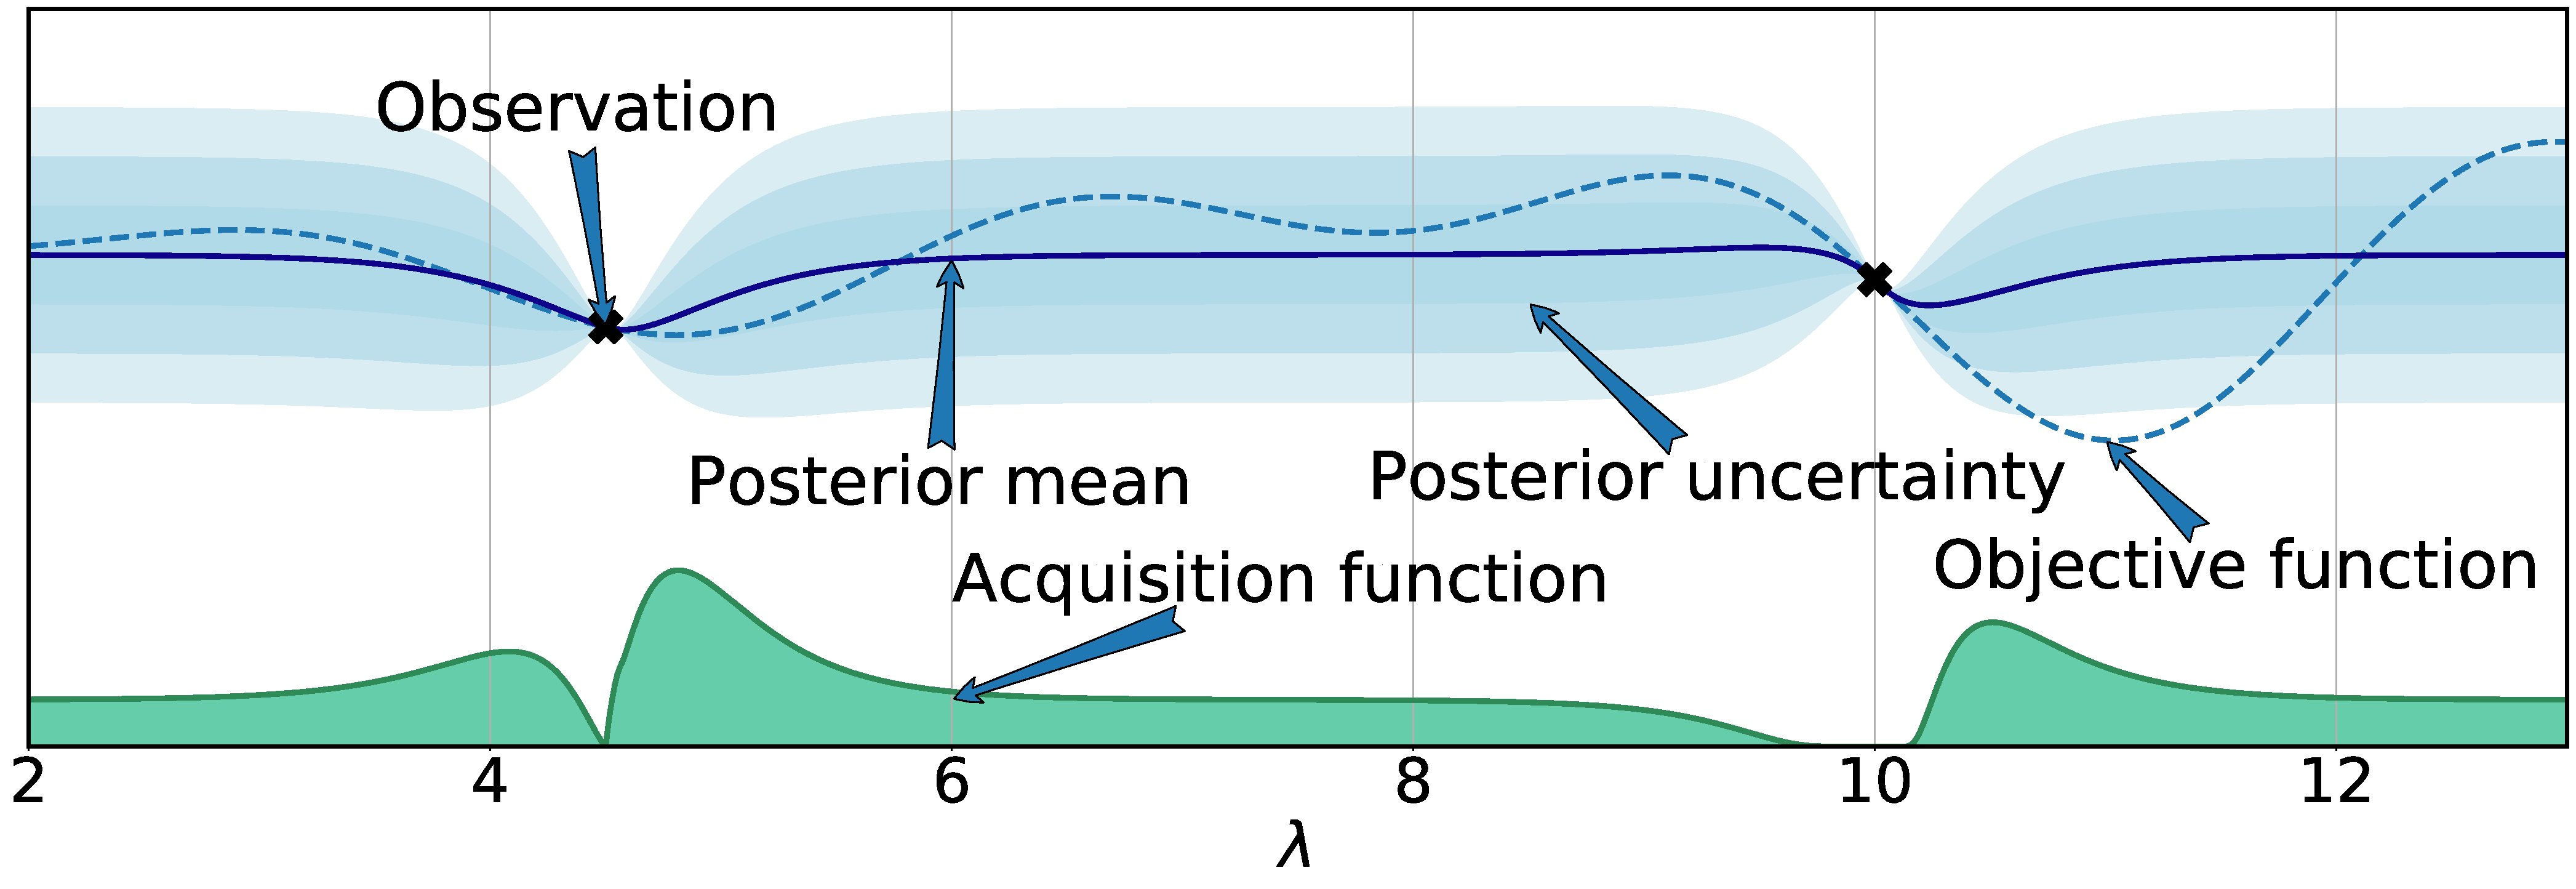
\includegraphics[width=0.95\textwidth]{images/intro_images/IntroPlots_Acqui.pdf}
        }\only<4->{
            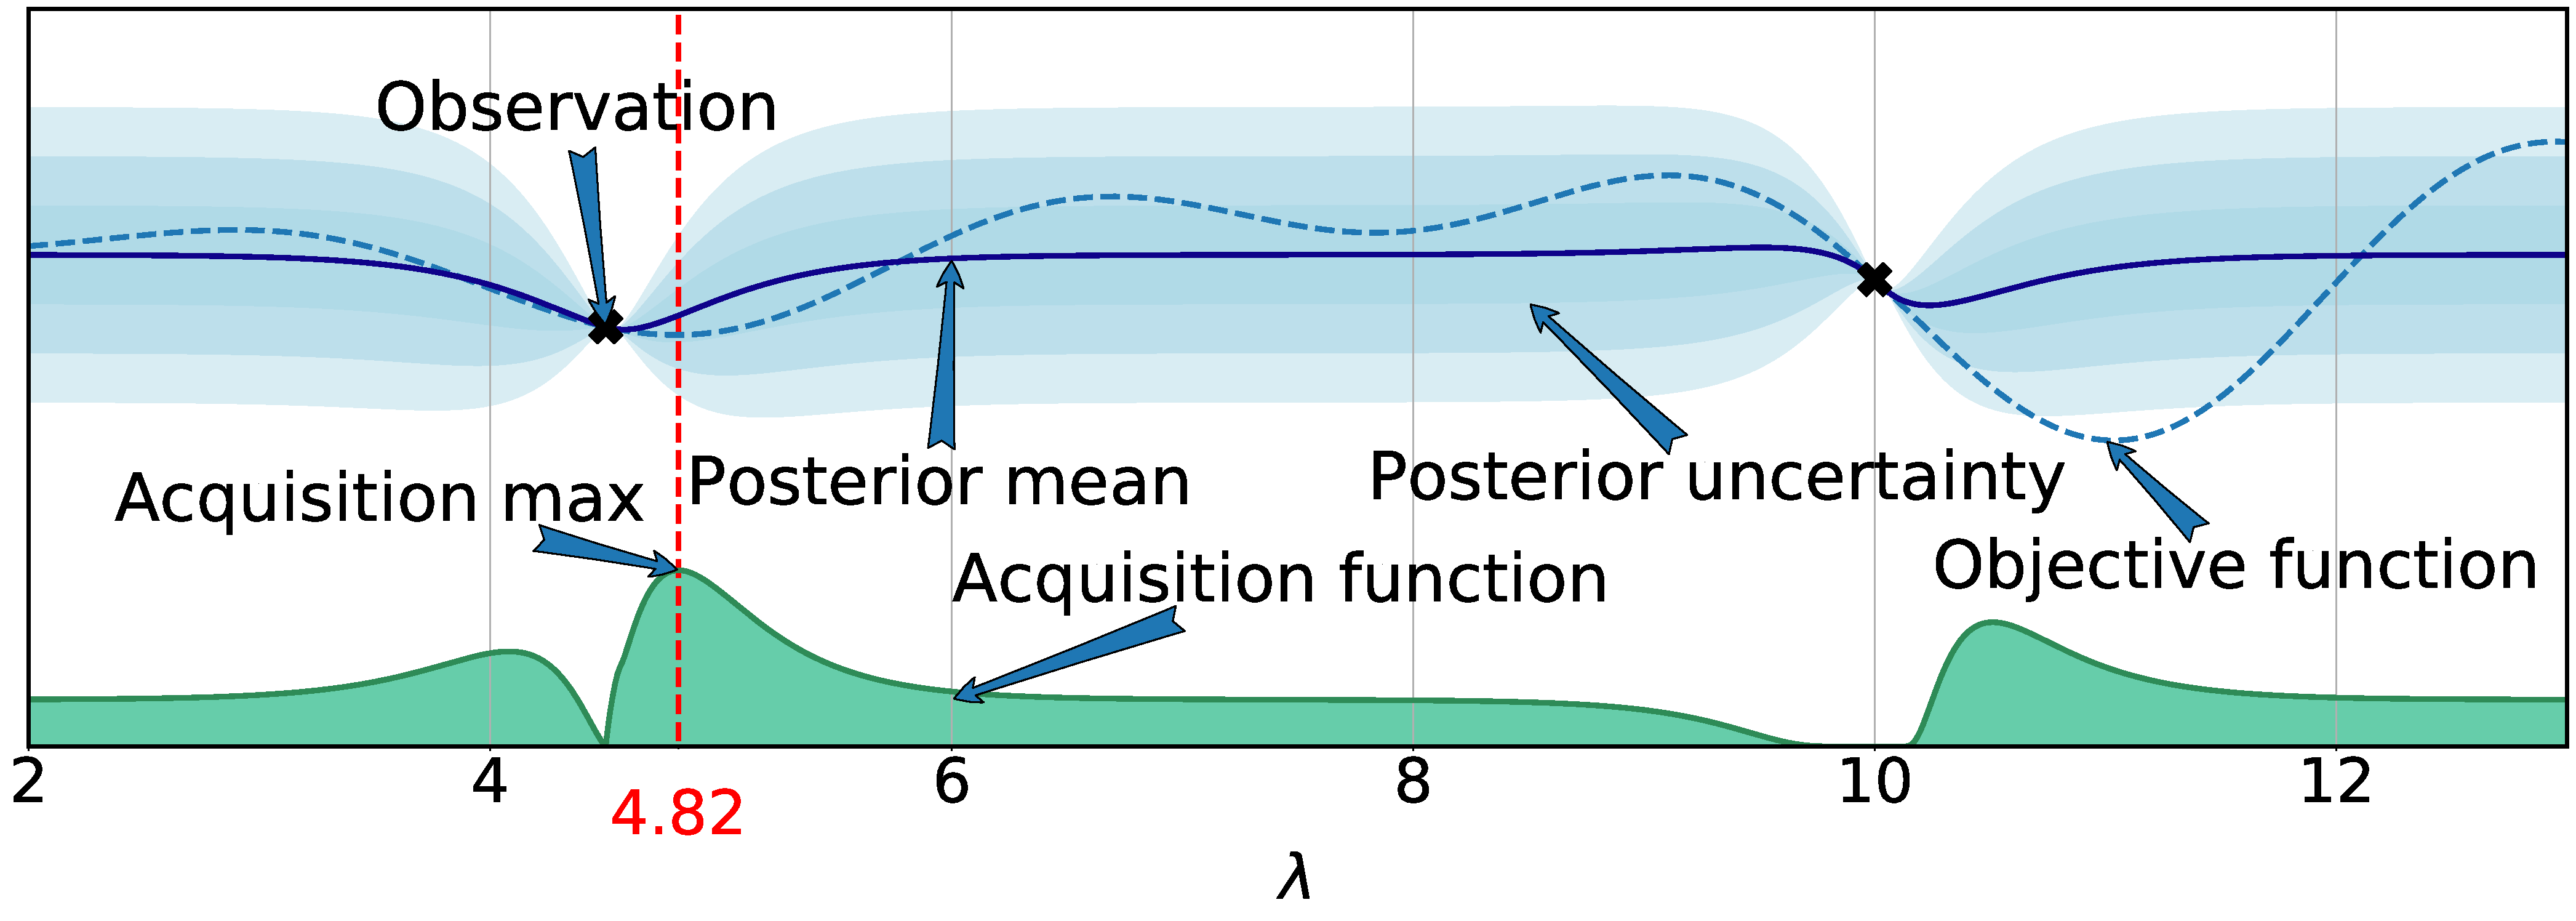
\includegraphics[width=0.95\textwidth]{images/intro_images/IntroPlots_Complete.pdf}
        }
    \end{figure}
    
% \vspace*{-0.5cm}\notefh{Can you please increase the plotted values of the acquisition function, so that it is more clearly visible? Also on the next slide. You could, e.g., normalize it to have a certain maximum (a bit larger than that of the third plot on the next slide). Also, on the next slide, can you please plot the new observation red, not green?}
}

%----------------------------------------------------------------------
\begin{frame}[c]{Bayesian Optimization of a blackbox function in a nutshell}

\begin{columns}[T]
\column{0.45\textwidth}
General approach
\begin{itemize}
    \item Fit a \alert{probabilistic model} to the collected function samples $\langle{}\conf, \cost(\conf)\rangle{}$
    \item Use the model to guide optimization, trading off \alert{exploration \vs{} exploitation}
%    \item Acquisition function for exploration-exploitation tradeoff
%    \item Optimize on acquisition function\\ to get next $x$ $\conf$ ($x$)
\end{itemize}

\bigskip

\onslide<4->{
    \alert{Popular approach in the statistics literature} since
    \lit{\href{http://link.springer.com/chapter/10.1007\%2F3-540-07165-2_55}{Mockus. 1975}}
    \begin{itemize}
        \item Efficient in \#function evaluations
        \item Works when objective is \alert{nonconvex, noisy, has unknown derivatives, etc.}
        \item Recent \alert{convergence} results\\ \lit{\href{https://arxiv.org/pdf/0912.3995.pdf}{Srinivas et al. 2009}; \href{http://www.jmlr.org/papers/v12/bull11a.html}{Bull. 2011}; \href{https://www.cs.ubc.ca/~nando/papers/BayesBandits.pdf}{de Freitas et al. 2012}; \href{https://proceedings.neurips.cc/paper/2015/file/0ebcc77dc72360d0eb8e9504c78d38bd-Paper.pdf}{Kawaguchi et al. 2015}}
    %    \item Popular \alert{Bayesian optimization workshop} at NIPS (the premiere machine learning conference)
    \end{itemize}
}

\column{0.55\textwidth}
\onslide<1->
\begin{figure}
    \vspace{-1em}
    \centering
    \onslide<1->{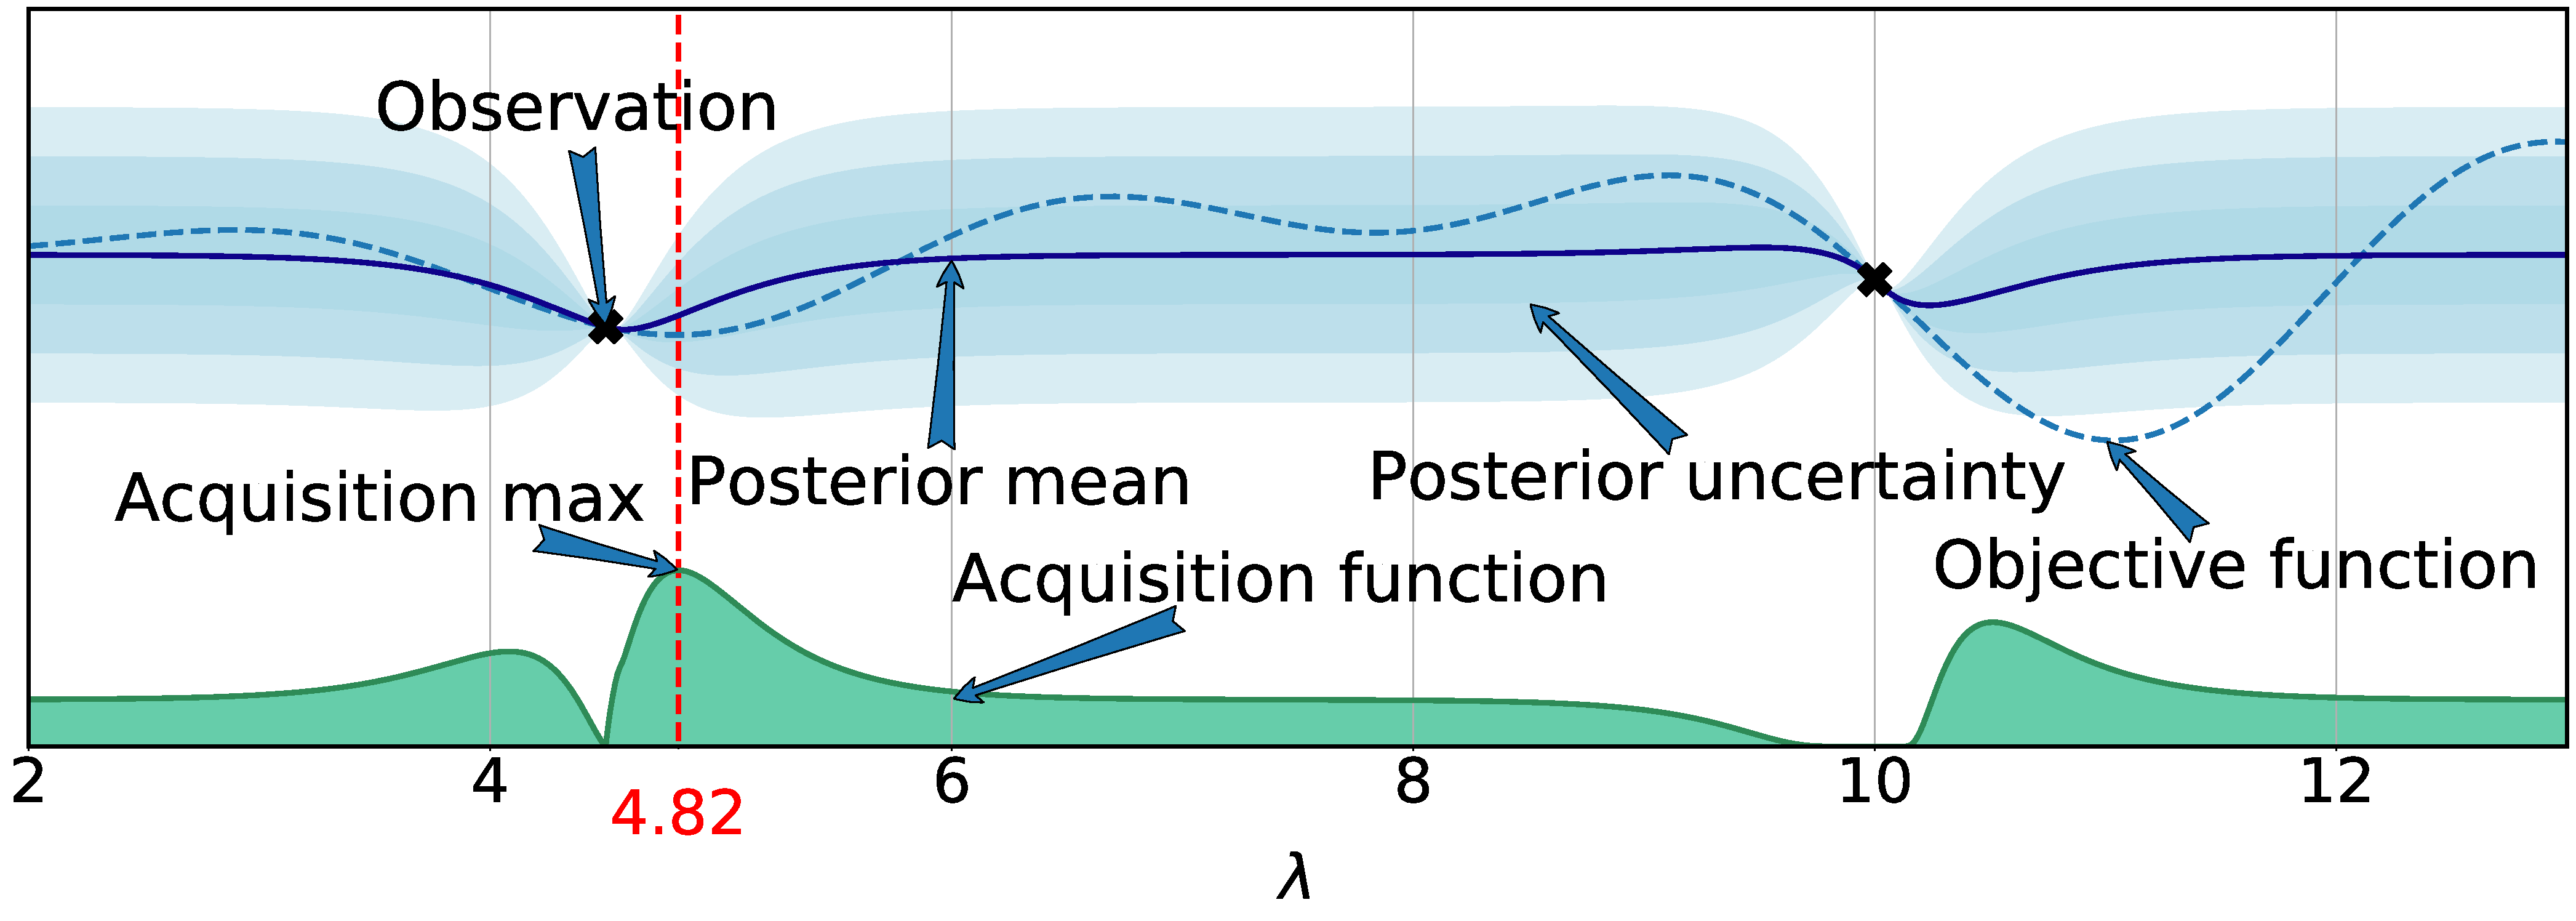
\includegraphics[width=0.8\textwidth]{images/intro_images/IntroPlots_Iter2.pdf}}
    \onslide<2->{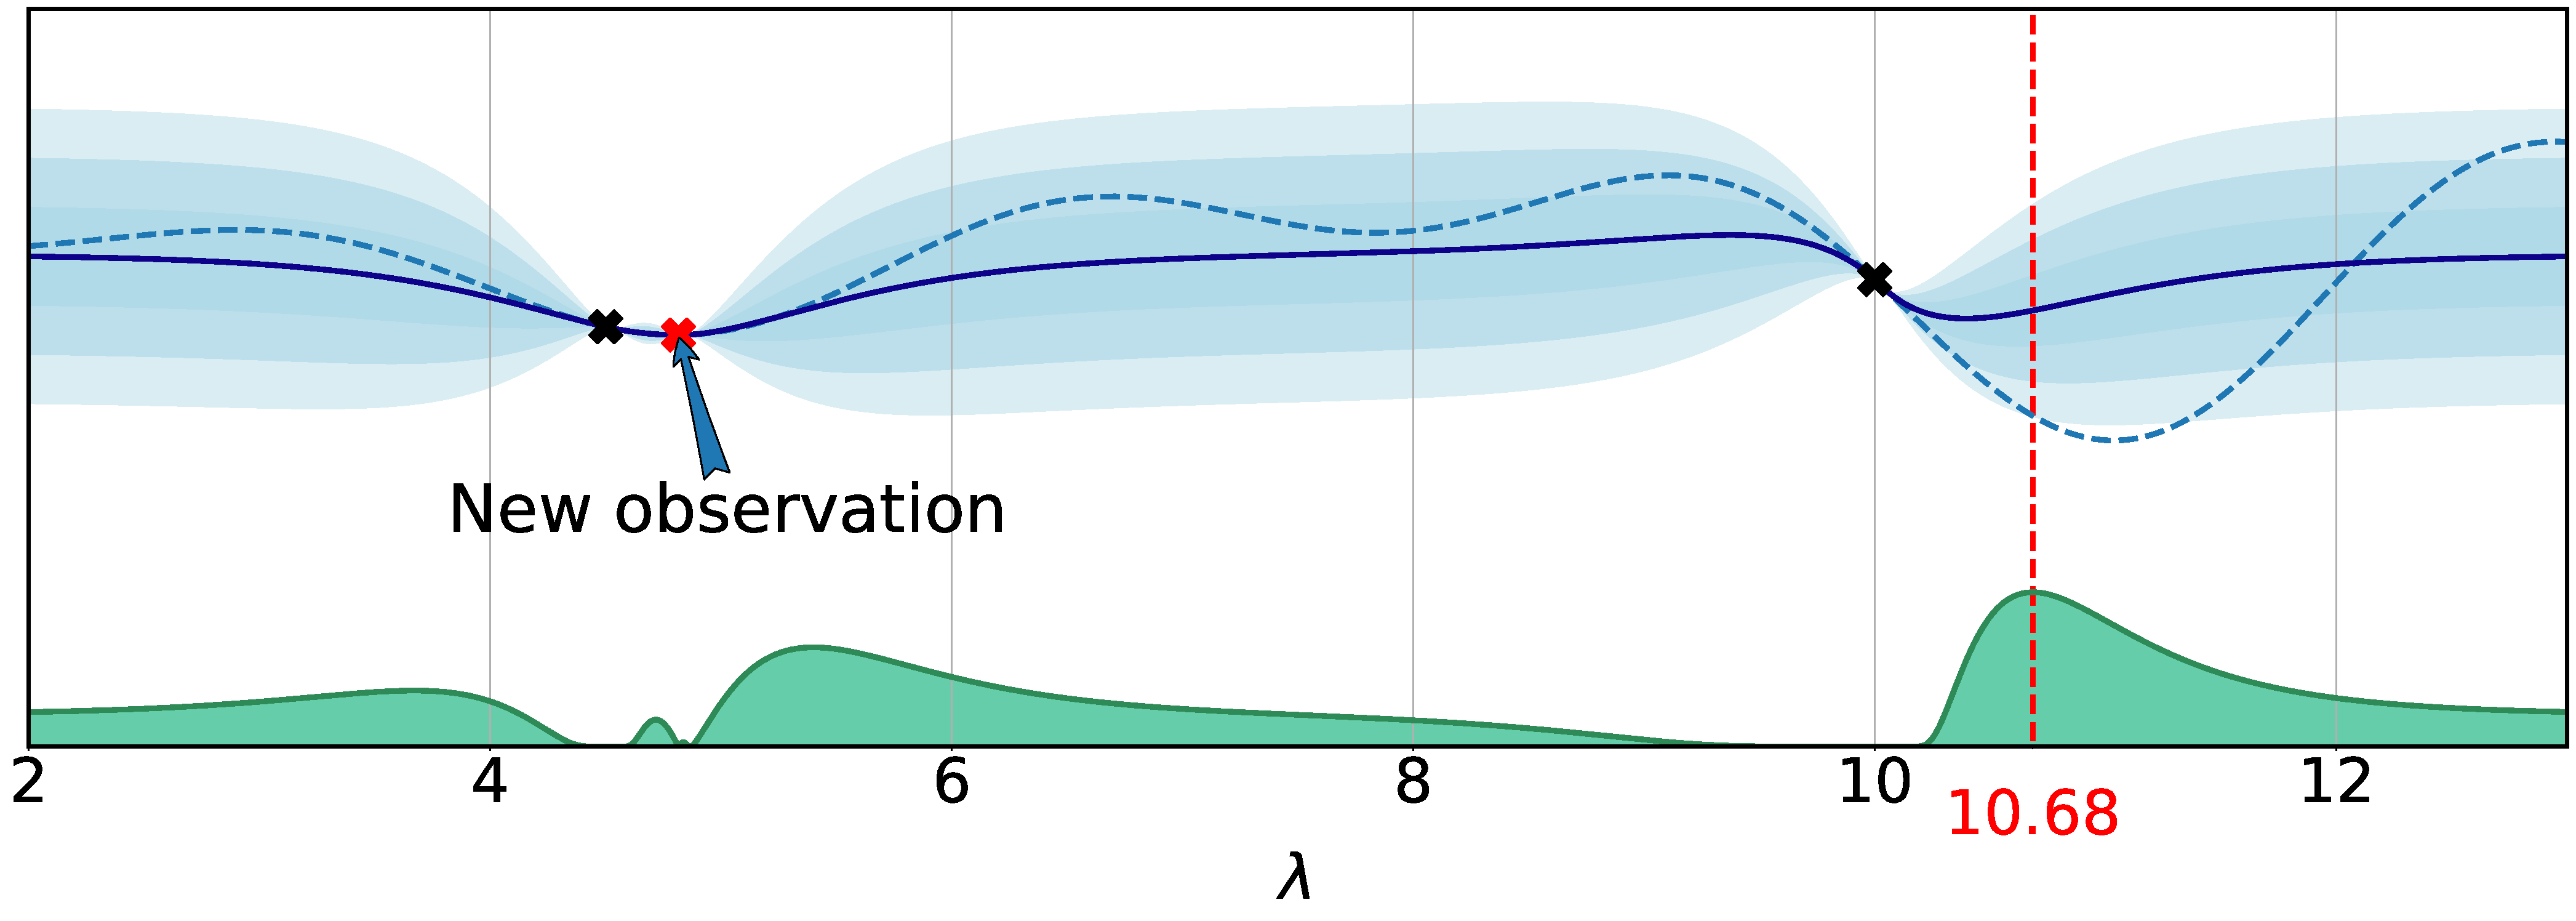
\includegraphics[width=0.8\textwidth]{images/intro_images/IntroPlots_Iter3.pdf}}
    \onslide<3->{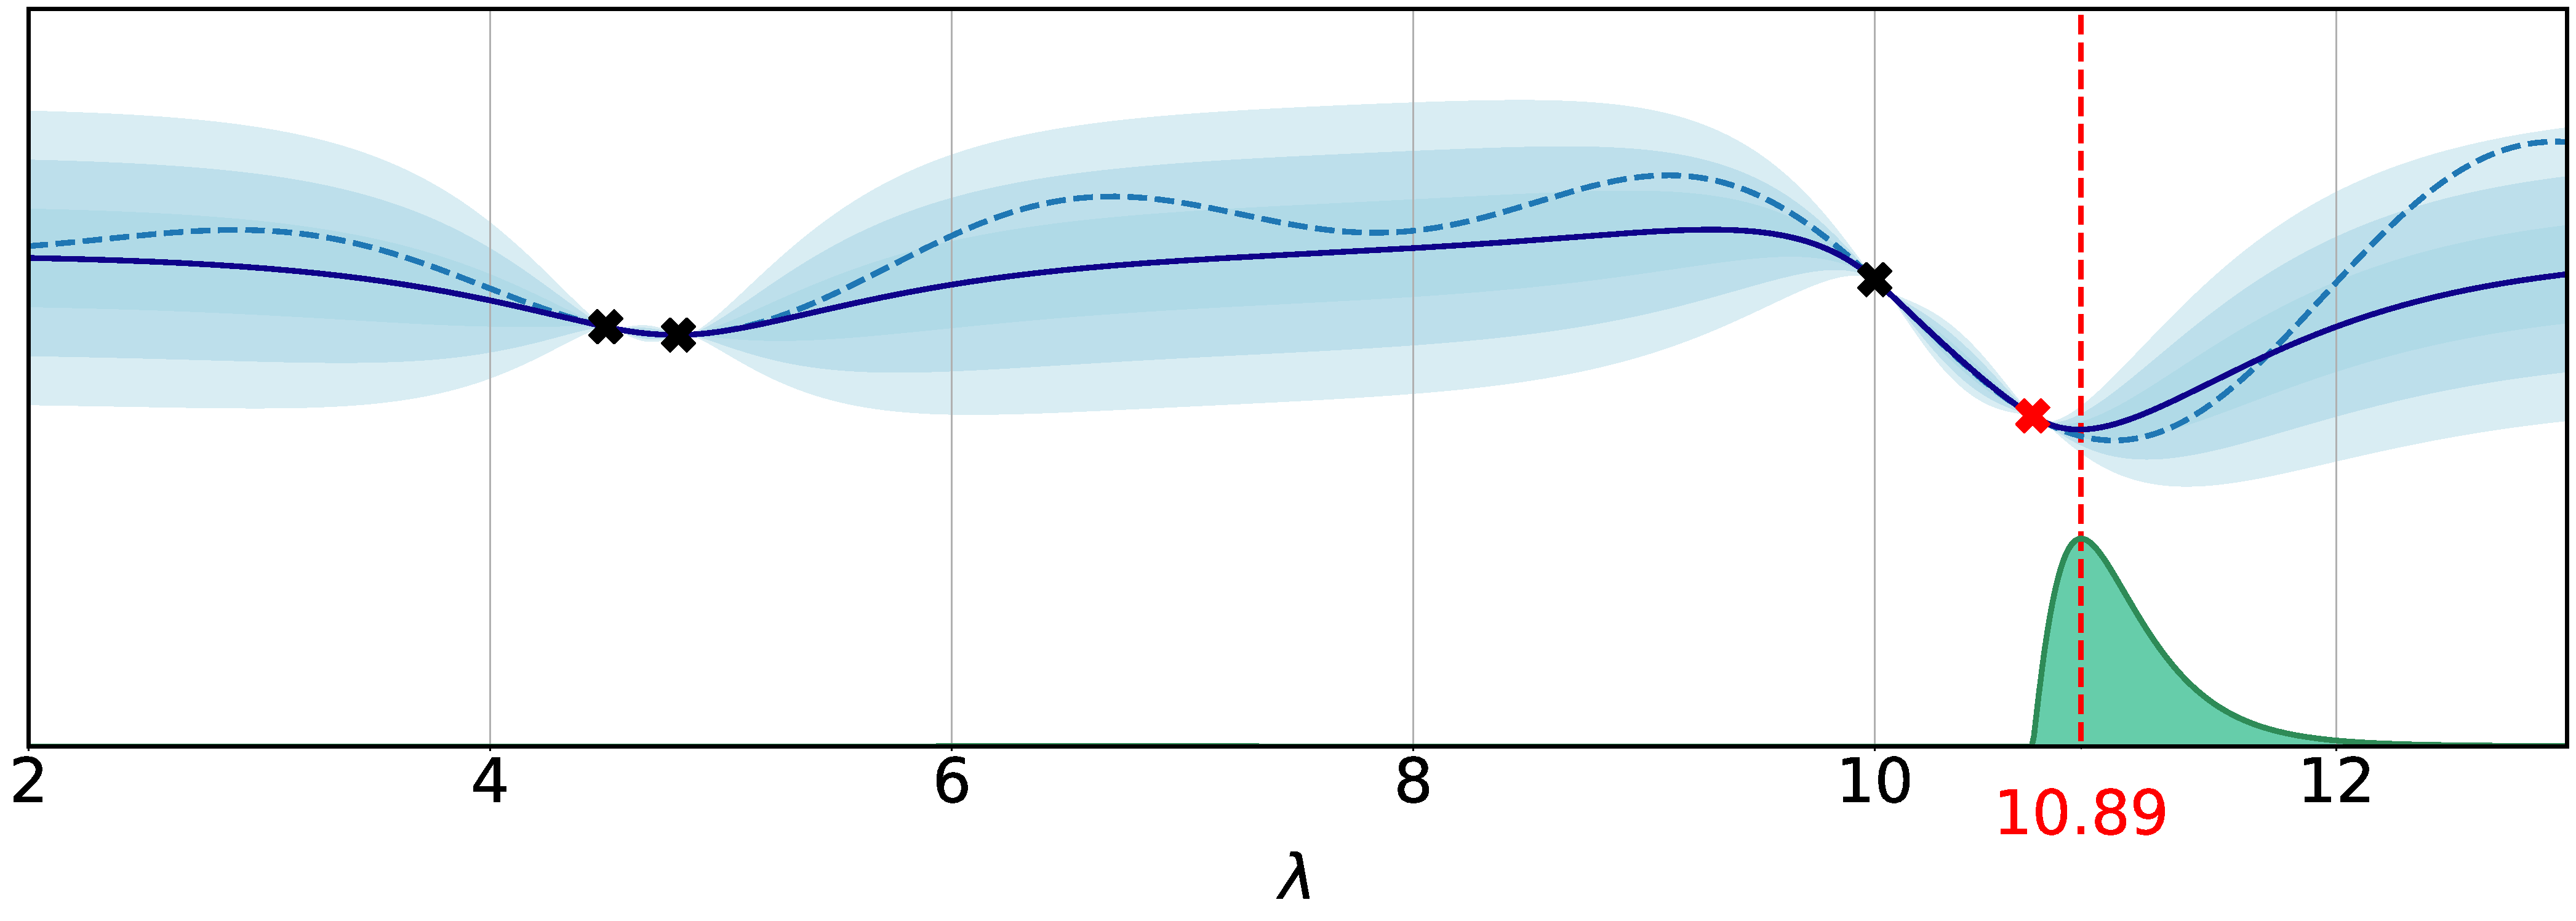
\includegraphics[width=0.8\textwidth]{images/intro_images/IntroPlots_Iter4.pdf}}
    %\only<4>{\includegraphics[width=\textwidth]{images/intro_images/plot_2.pdf}}
    %\only<5>{\includegraphics[width=\textwidth]{images/intro_images/plot_3.pdf}}
    %\only<6>{\includegraphics[width=\textwidth]{images/intro_images/plot_4.pdf}}
    %\only<7>{\includegraphics[width=\textwidth]{images/intro_images/plot_5.pdf}}
    %\only<8>{\includegraphics[width=\textwidth]{images/intro_images/plot_6.pdf}}
    %\only<9->{\includegraphics[width=\textwidth]{images/intro_images/plot_7.pdf}}
\end{figure}
\end{columns}

\end{frame}
%-----------------------------------------------------------------------
%\myframe{Bayesian Optimization in a Nutshell}{
%  
%\vspace*{-0.5cm}
%\begin{columns}[T]
%
%\column{0.6\textwidth}
%
%\myblock{General approach}{
%	\myit{
%	  \item Fit a probabilistic model to the collected function samples
%	  $\langle{}\conf, \cost(\conf)\rangle{}$
%	  \item Use the model to guide optimization, trading off
%	  exploration \vs{} exploitation
%	%  \item Acquisition function for exploration-exploitation tradeoff
%	%  \item Optimize on acquisition function\\ to get next $x$
%	  %$\conf$ ($x$)
%	}
%}
%
%\smallskip
%\onslide<5->{
%	\myblock{Popular approach in the statistics literature since \litw{\href{http://link.springer.com/chapter/10.1007\%2F3-540-07165-2_55}{Mockus,
%	1978}}}{ \myit{
%		  	\item Efficient in \# function evaluations 
%		  	\item Works when objective is nonconvex, noisy, has unknown derivatives, etc
%			\fhpause
%			\item Recent convergence results\\ \lit{Srinivas et al, 2010; Bull 2011;
%			de Freitas et al, 2012; Kawaguchi et al, 2015}
%			%TODO: sorry, I don't know these papers
%		%	\item Popular \alert{Bayesian optimization workshop} at NIPS (the premiere machine learning conference)
%		}
%	}
%}
%%\begin{enumerate}
%%  \item Fit an empirical performance model (EPM) 
%%  \item Acquisition function for exploration-exploitation tradeoff
%%  \item Optimize on acquisition function\\ to get next $\conf$ ($x$)
%%\end{enumerate}
%
%\column{0.4\textwidth}
%\vspace*{0.5cm}
%\onslide<2->{
%	%\includegraphics[width=1\textwidth]{../images/bo.png}
%	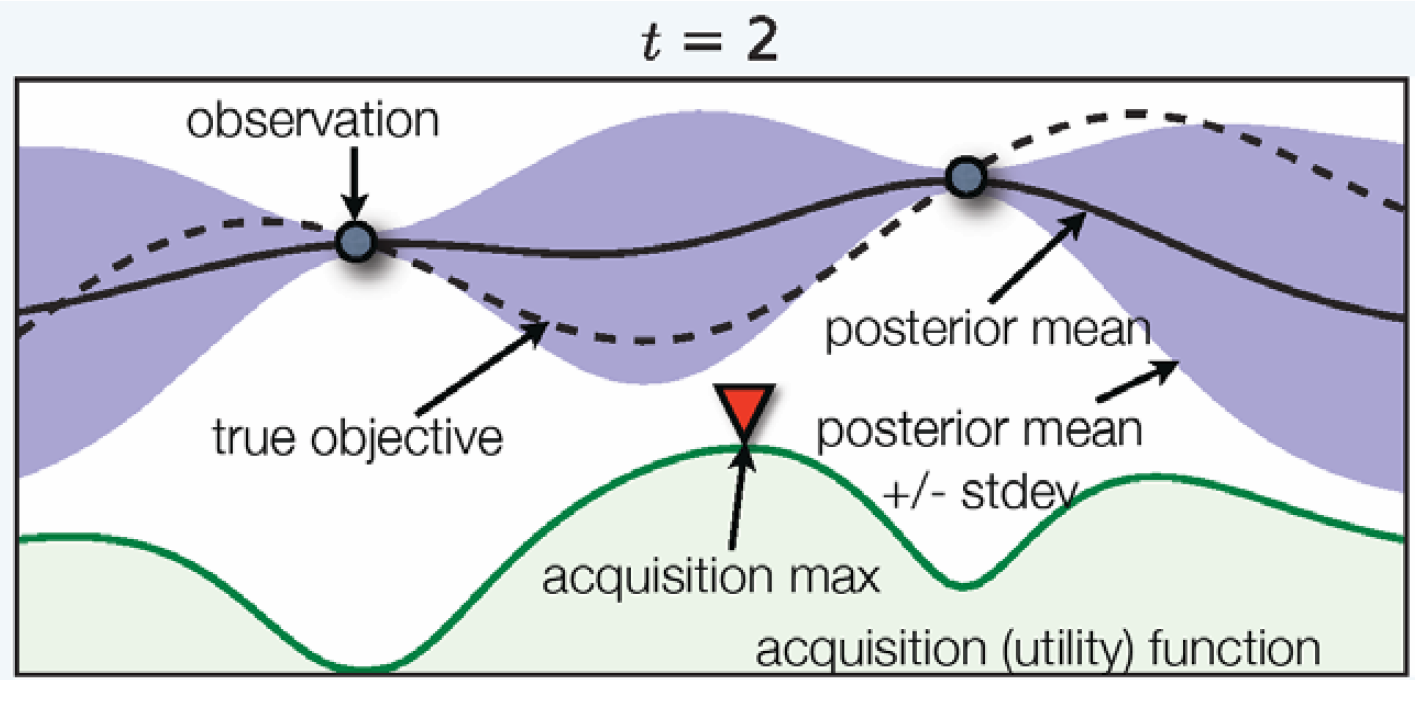
\includegraphics[width=0.9\textwidth]{plots_and_scripts/plots/bo_pic1.png}\\
%	\fhpause
%	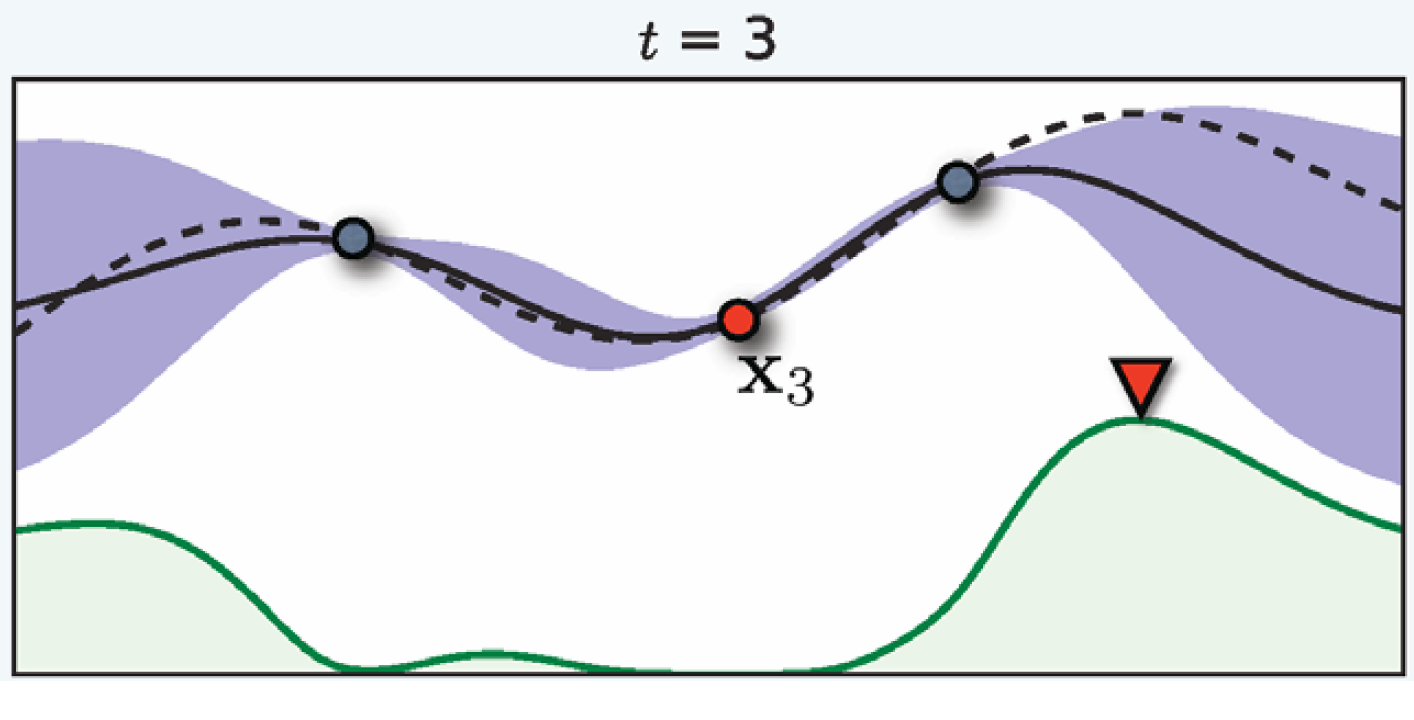
\includegraphics[width=0.9\textwidth]{plots_and_scripts/plots//bo_pic2.png}\\
%	\fhpause
%	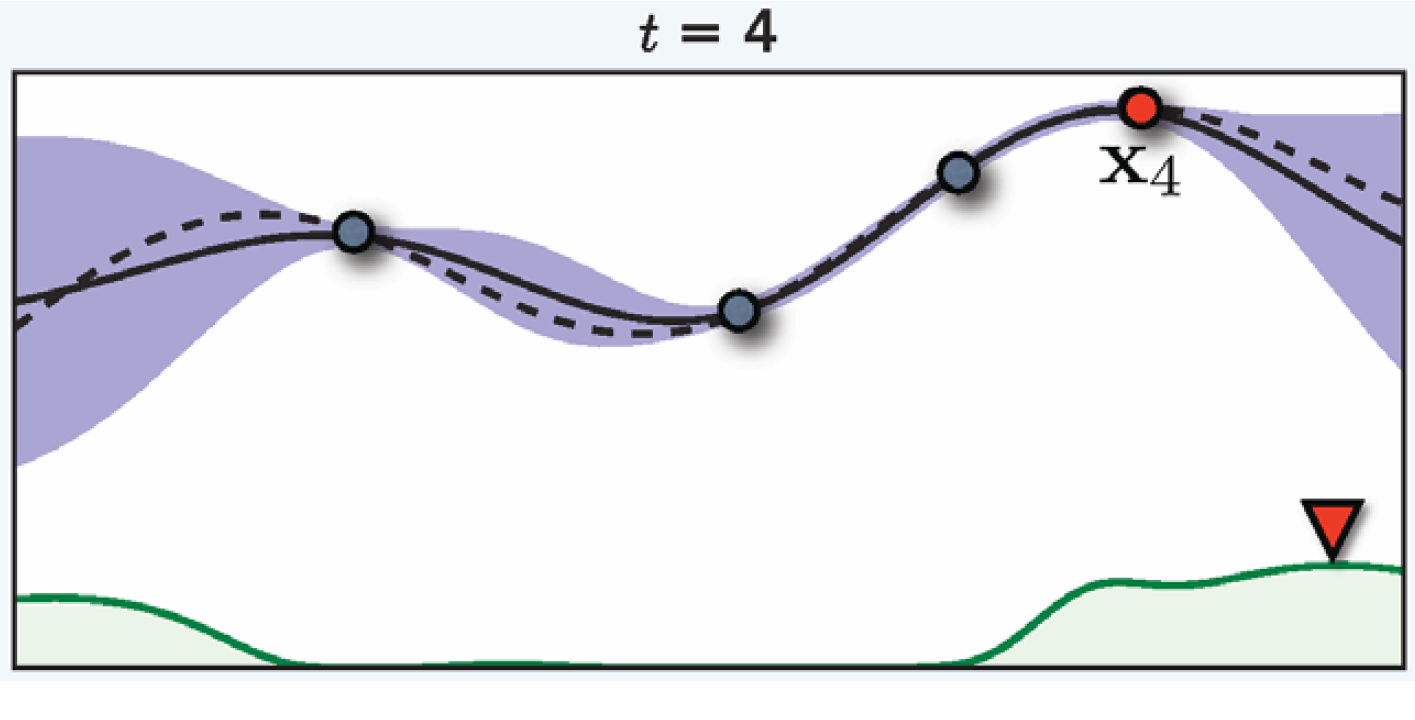
\includegraphics[width=0.9\textwidth]{plots_and_scripts/plots//bo_pic3.png}\\
%	\footnotesize{Image source: \lit{\href{https://arxiv.org/abs/1012.2599}{Brochu et al, 2010}}}
%}
%\end{columns}
%}
%----------------------------------------------------------------------
%5\begin{frame}[c]{Bayesian Optimization: Visualization of Many Steps}
%\begin{figure}
%    \centering
%    \only<1>{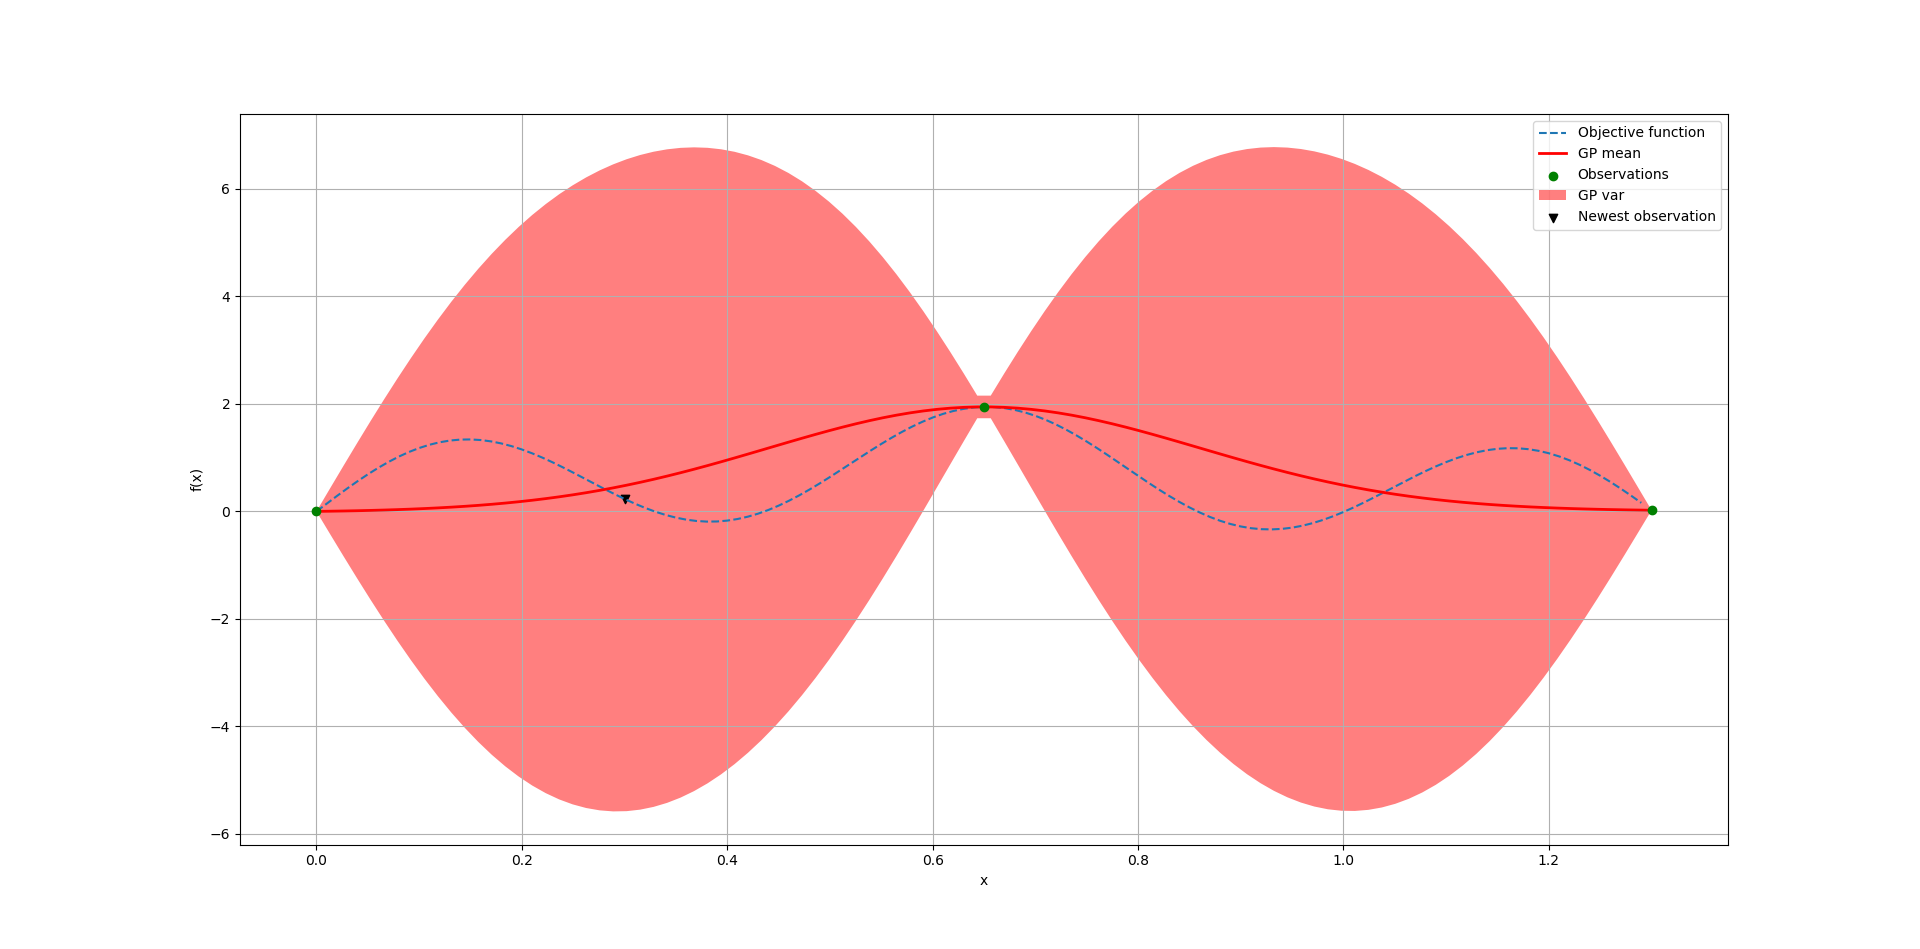
\includegraphics[width=\linewidth]{images/intro_images/BOLoop_1.png}}
%    \only<2>{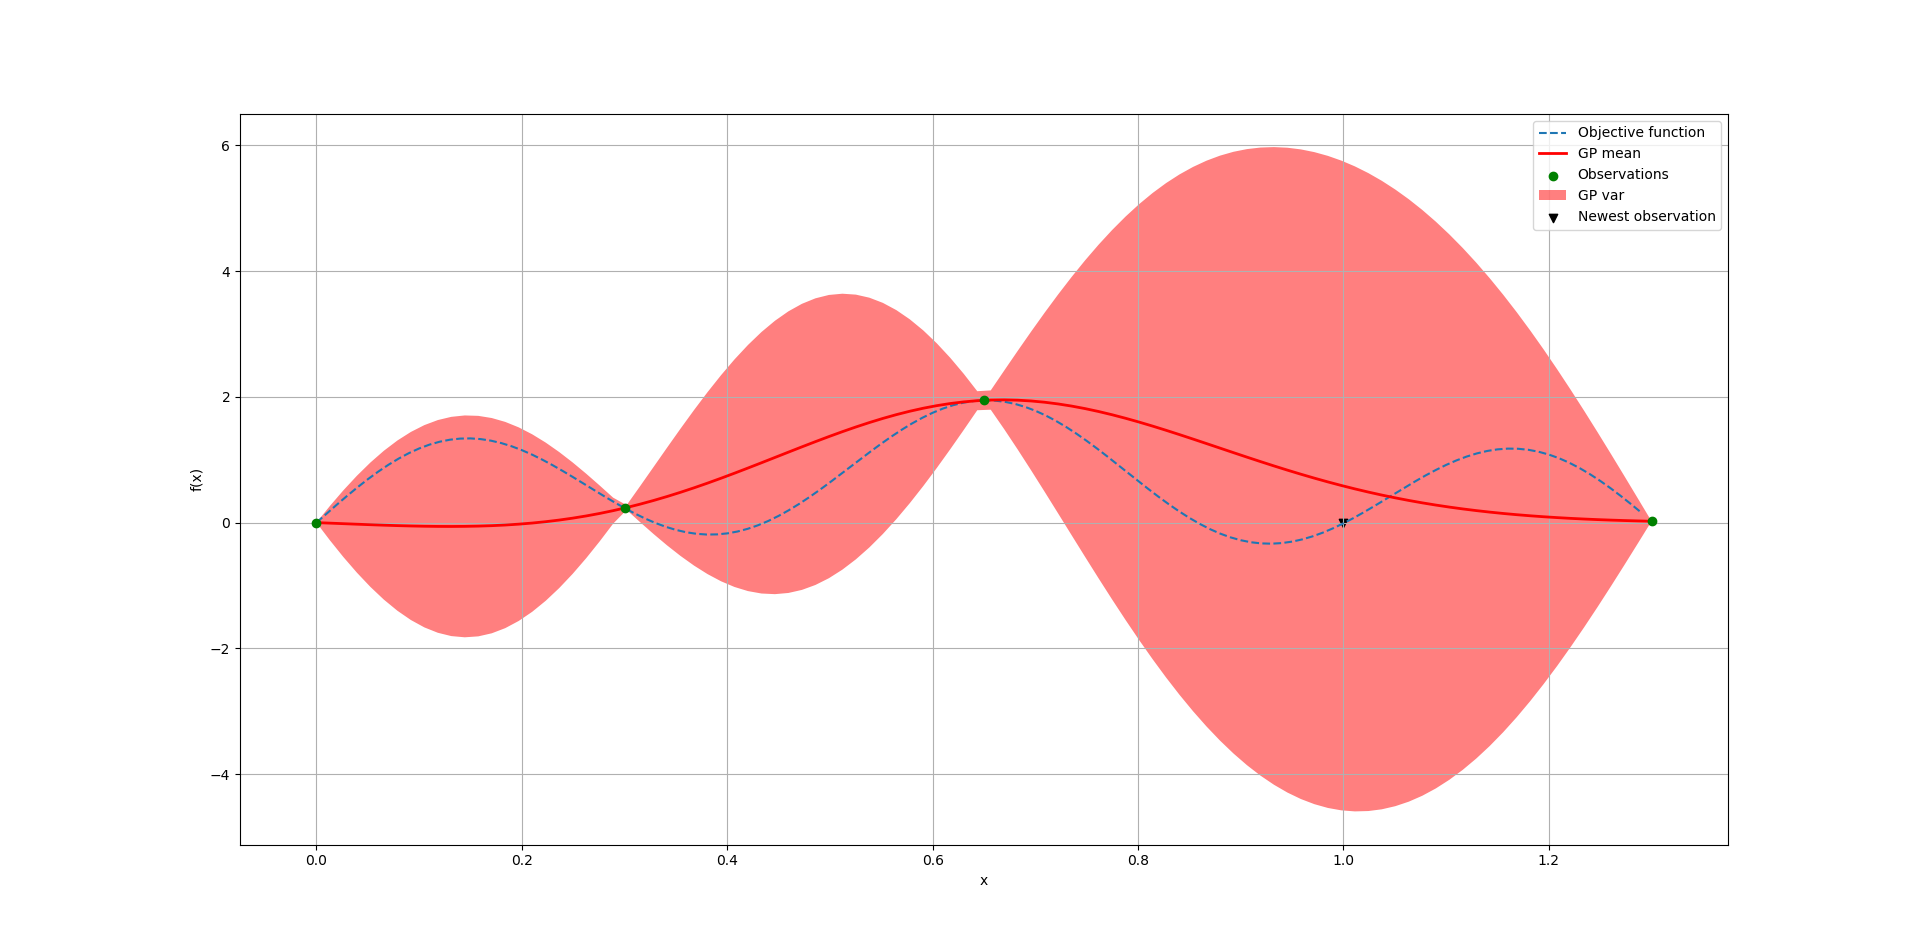
\includegraphics[width=\linewidth]{images/intro_images/BOLoop_2.png}}
%    \only<3>{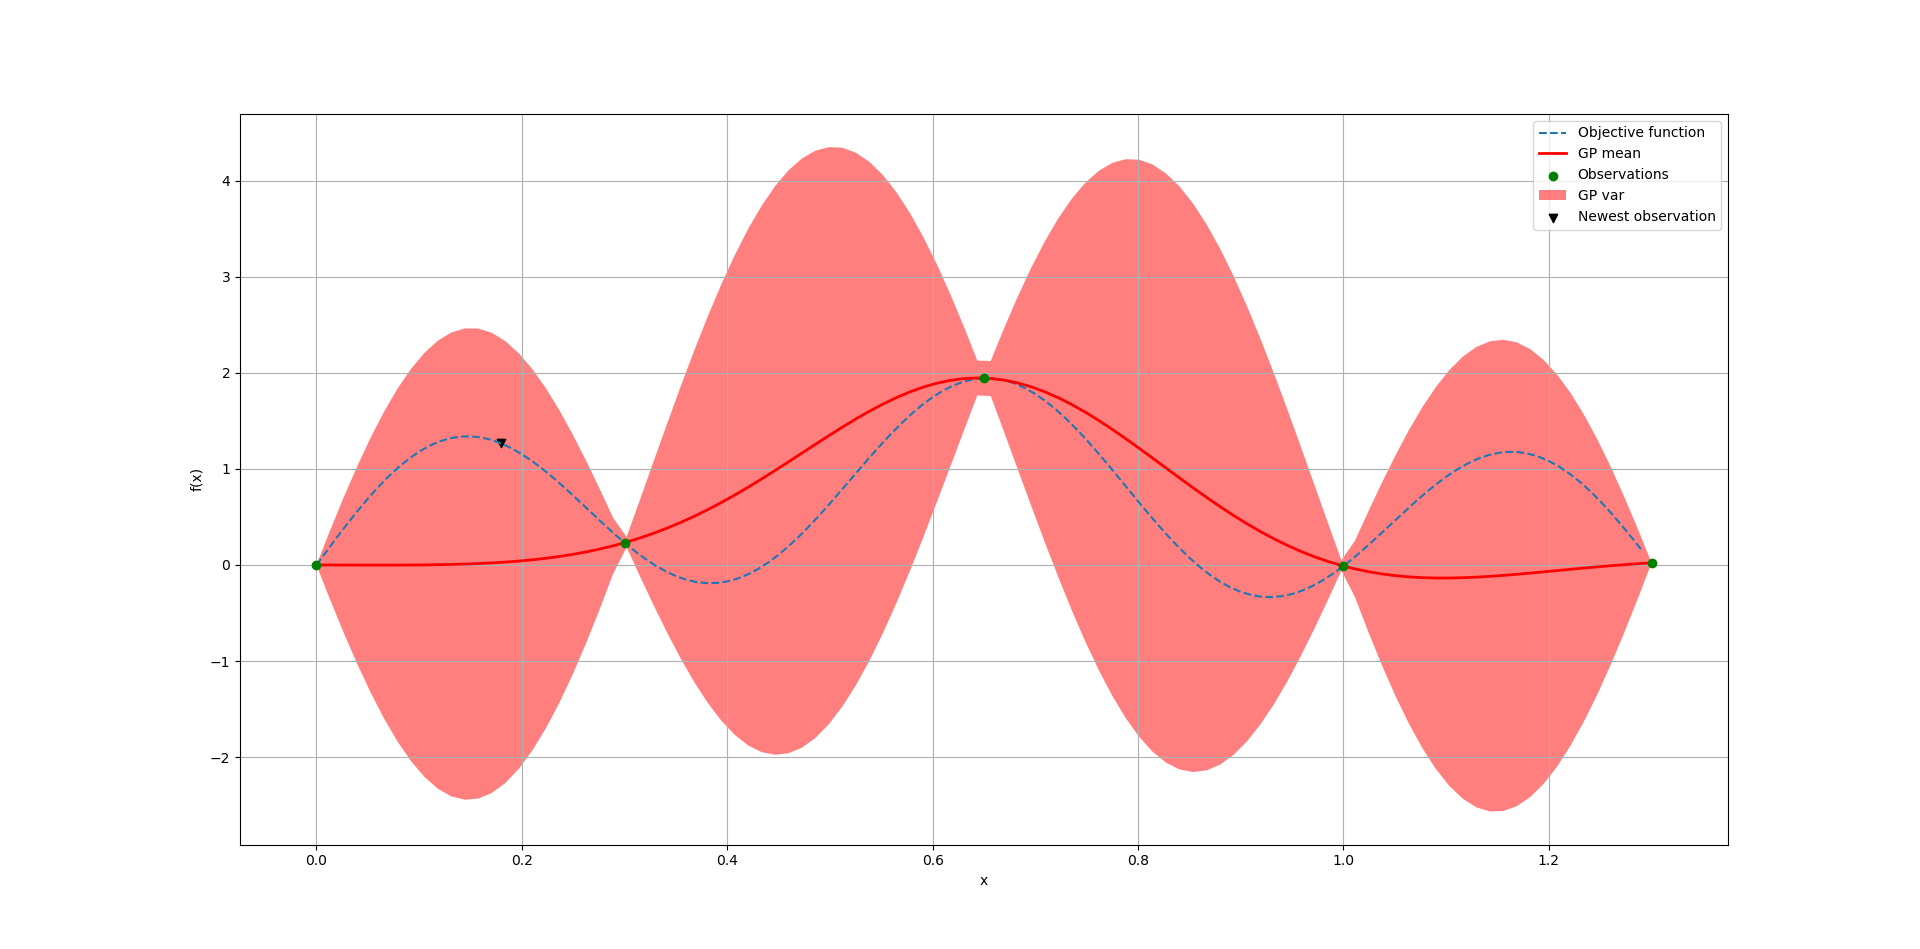
\includegraphics[width=\linewidth]{images/intro_images/BOLoop_3.png}}
%    \only<4>{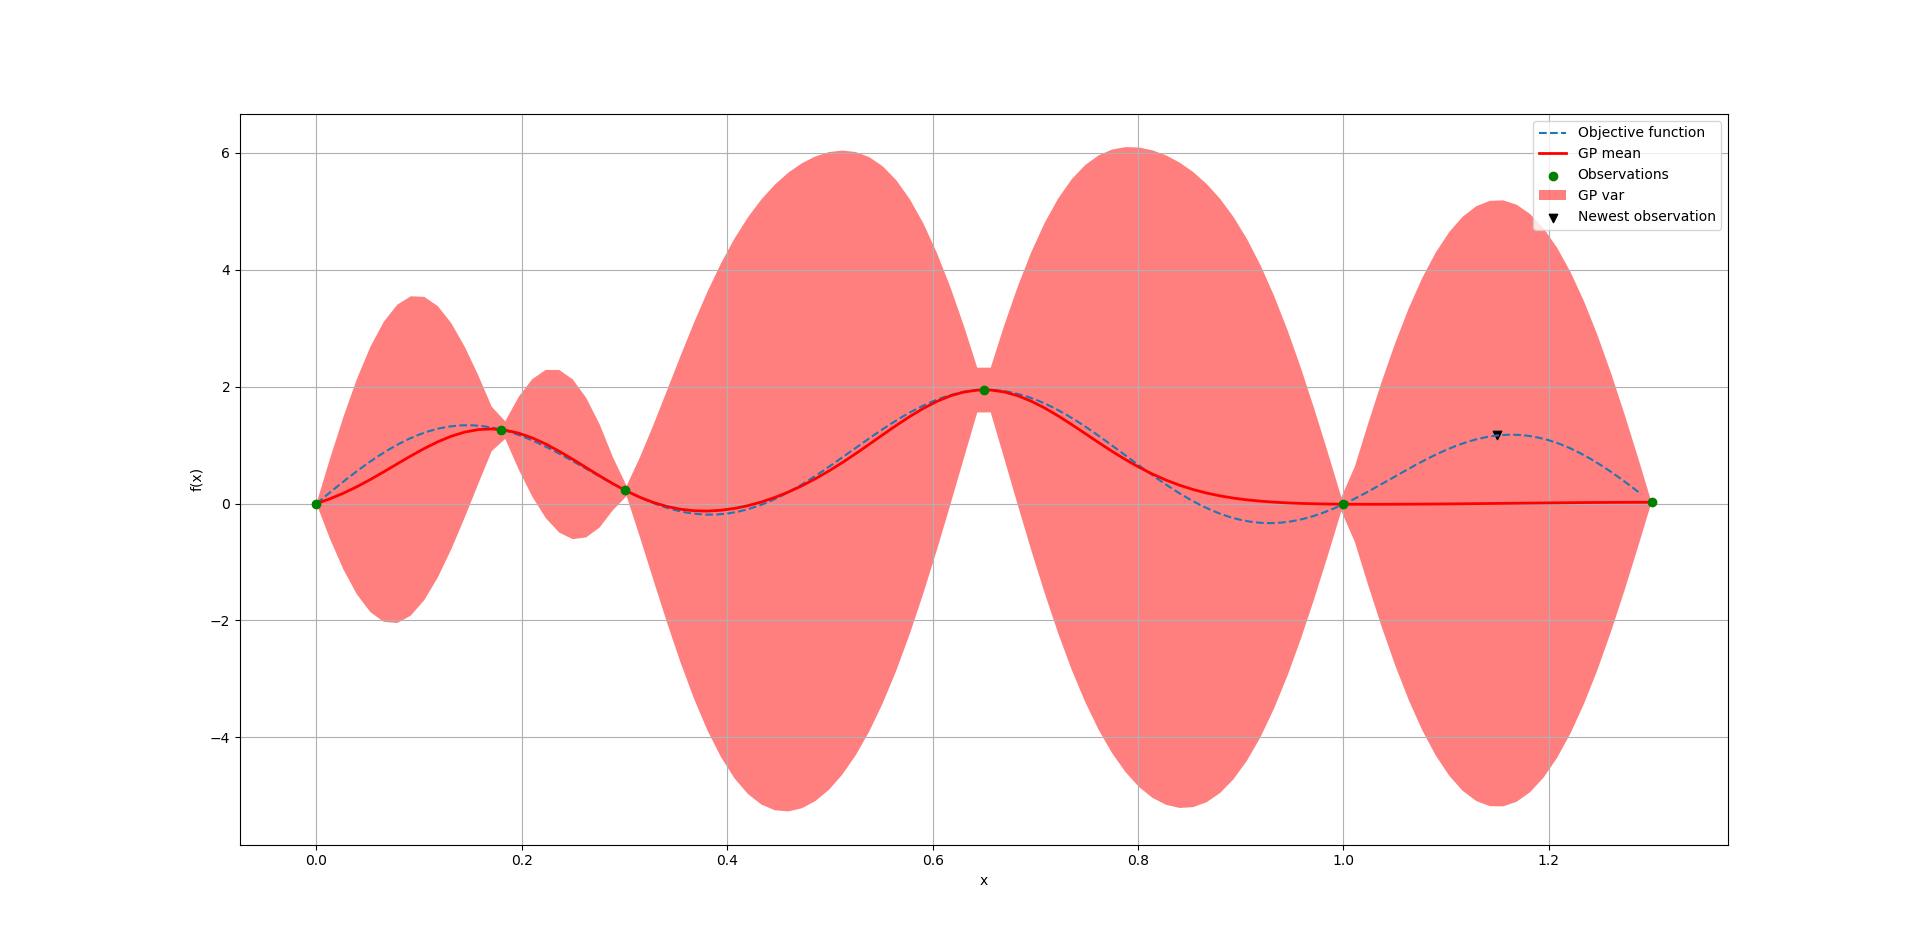
\includegraphics[width=\linewidth]{images/intro_images/BOLoop_4.png}}
%    \only<5>{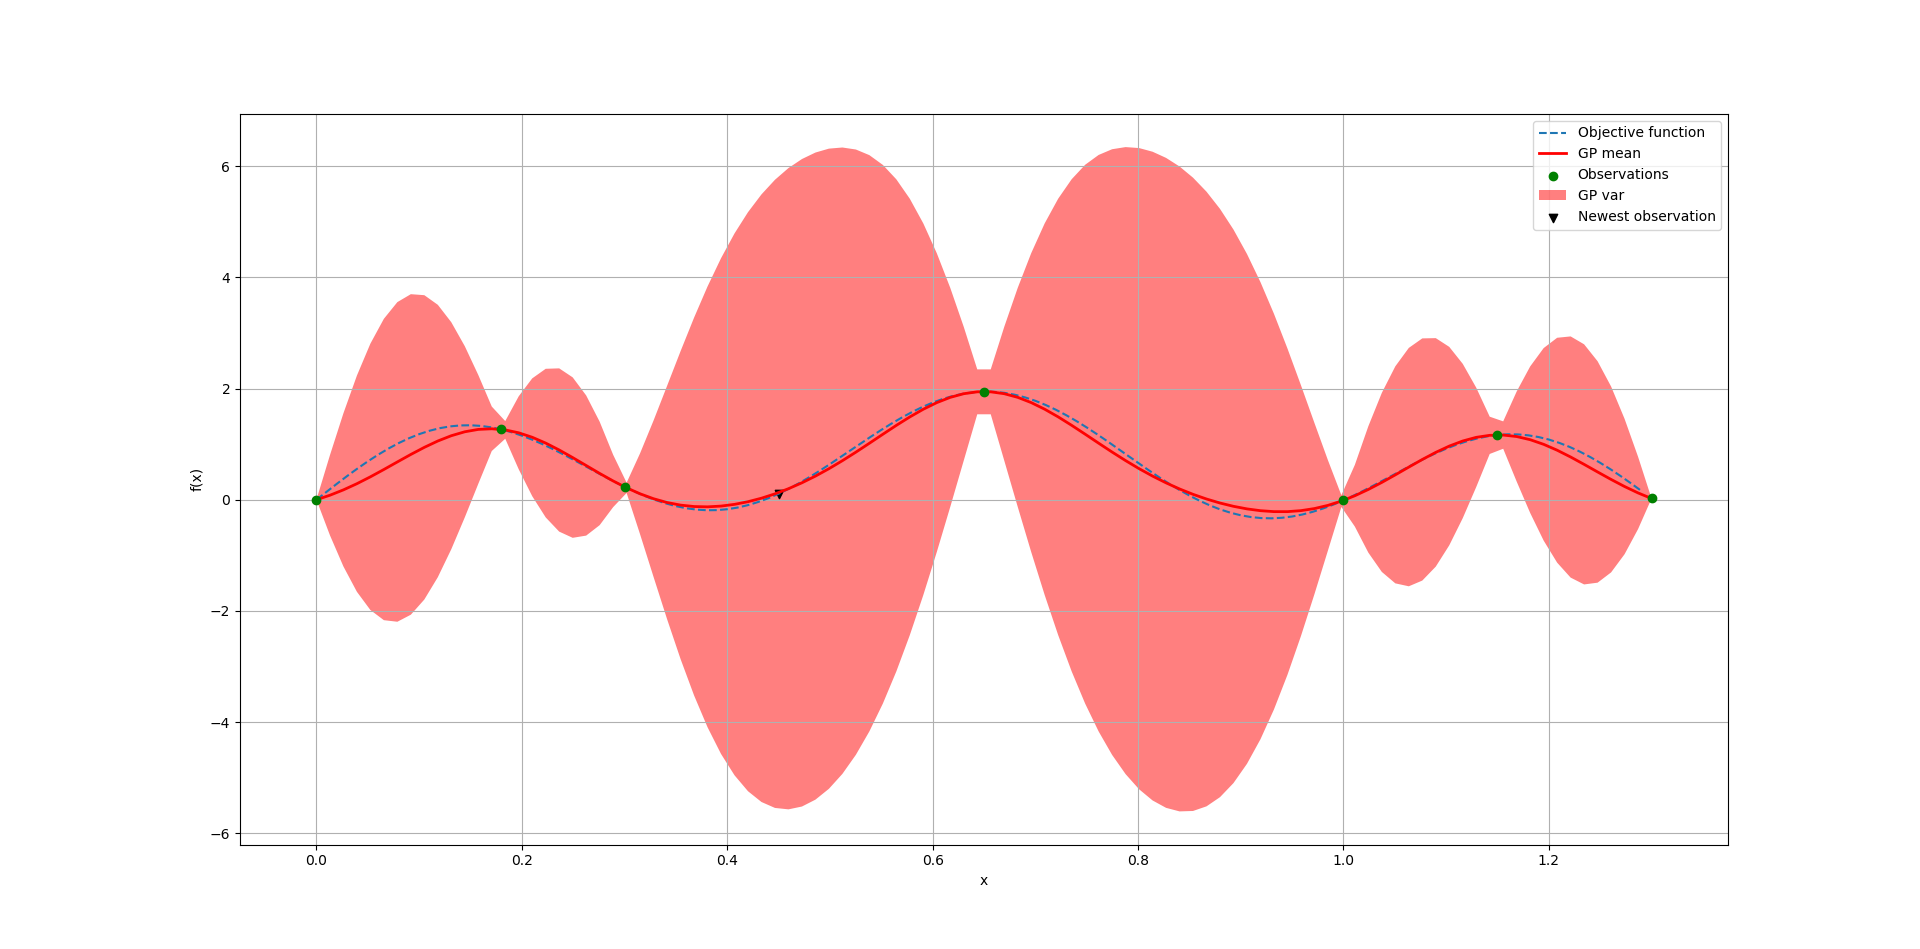
\includegraphics[width=\linewidth]{images/intro_images/BOLoop_5.png}}
%    \only<6>{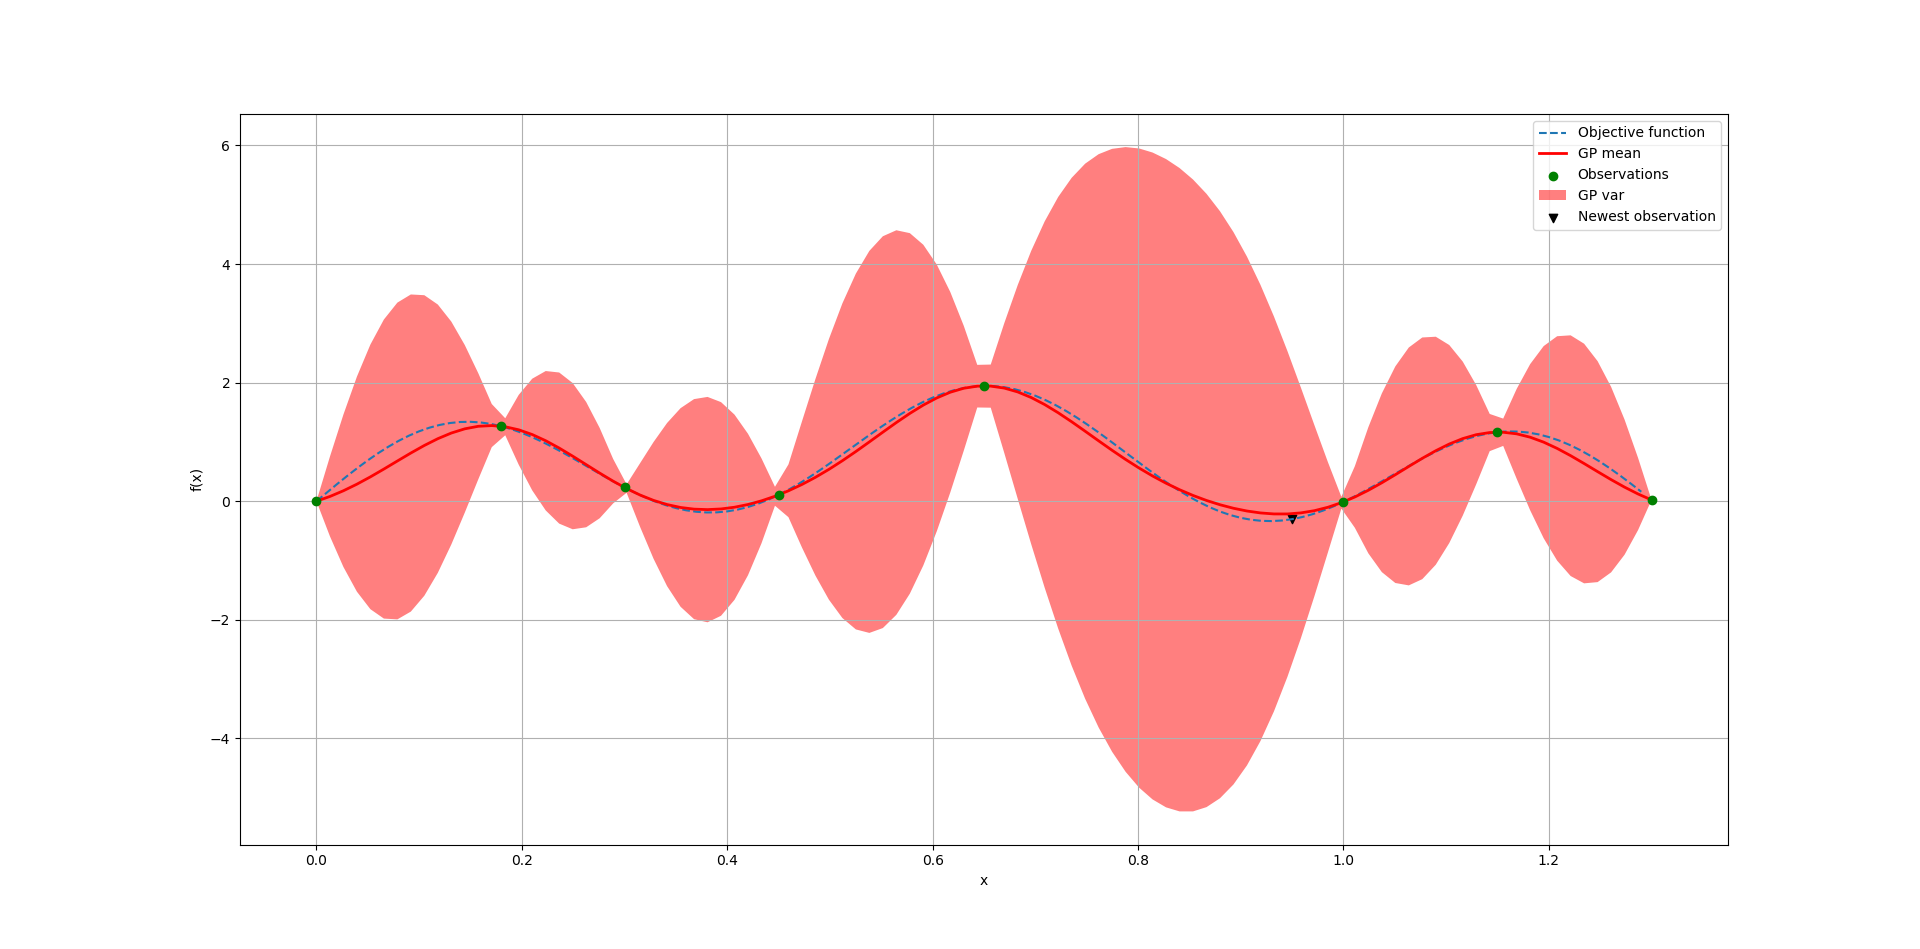
\includegraphics[width=\linewidth]{images/intro_images/BOLoop_6.png}}
%    \only<7>{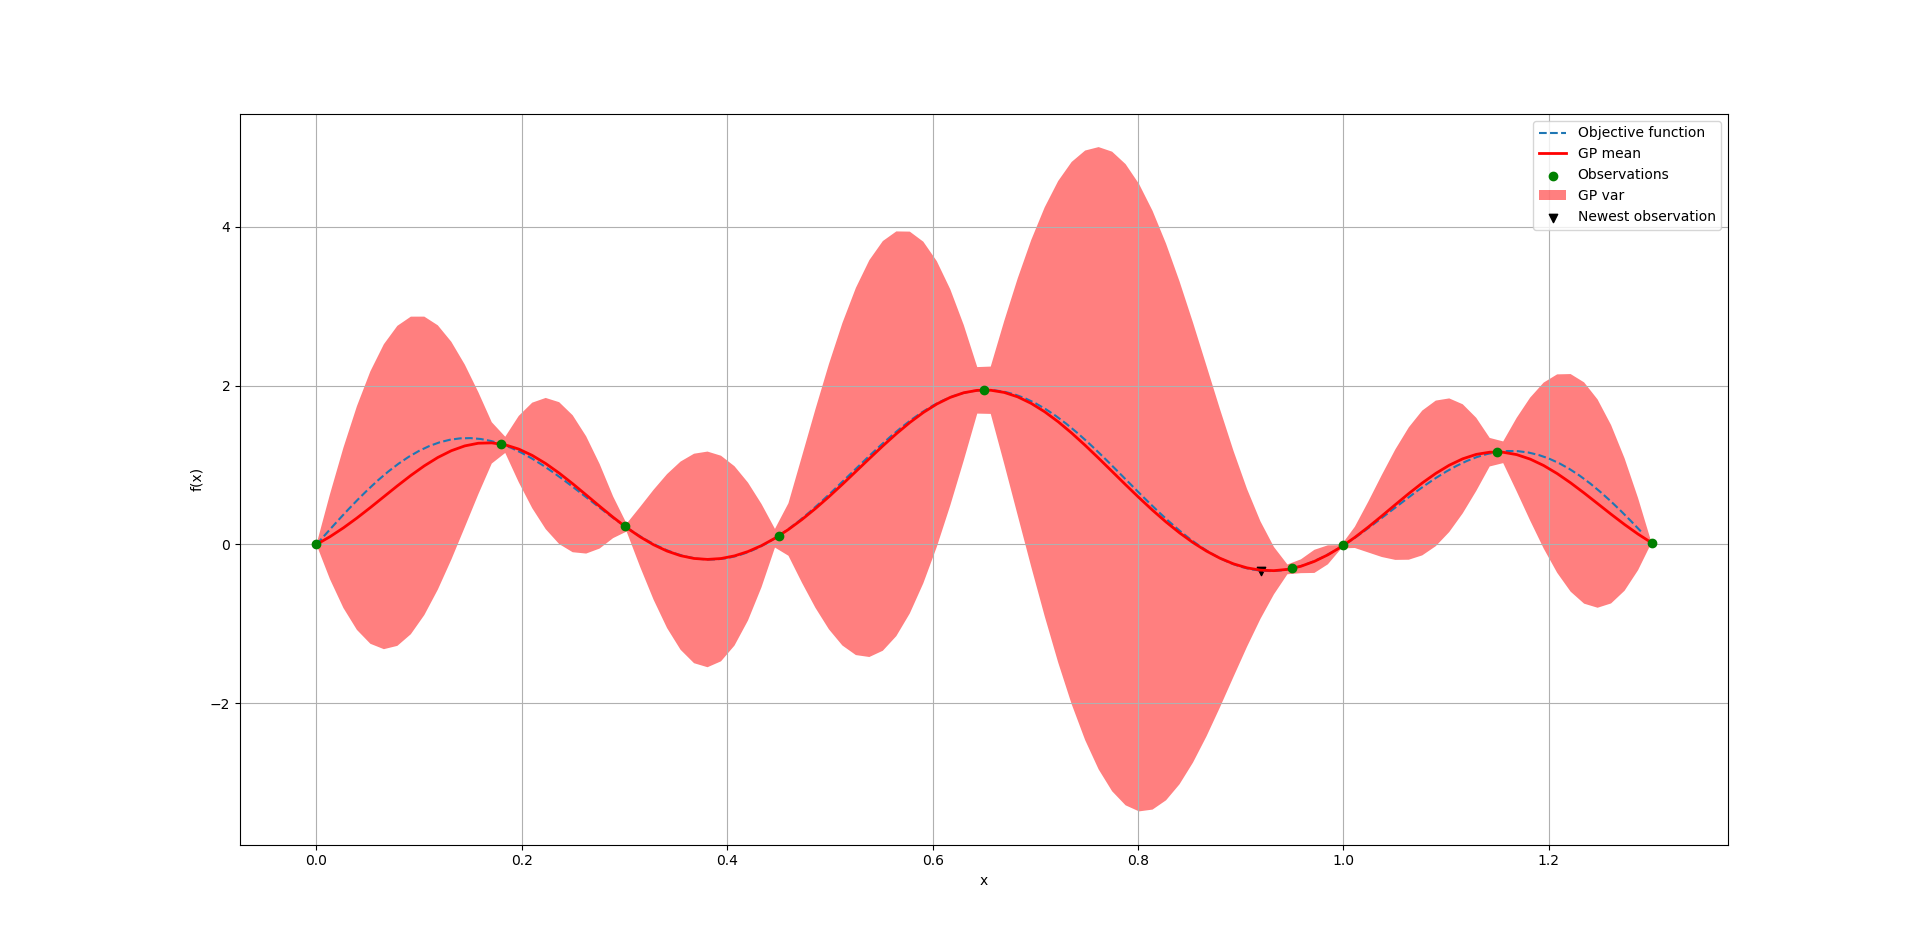
\includegraphics[width=\linewidth]{images/intro_images/BOLoop_7.png}}
%    \only<8>{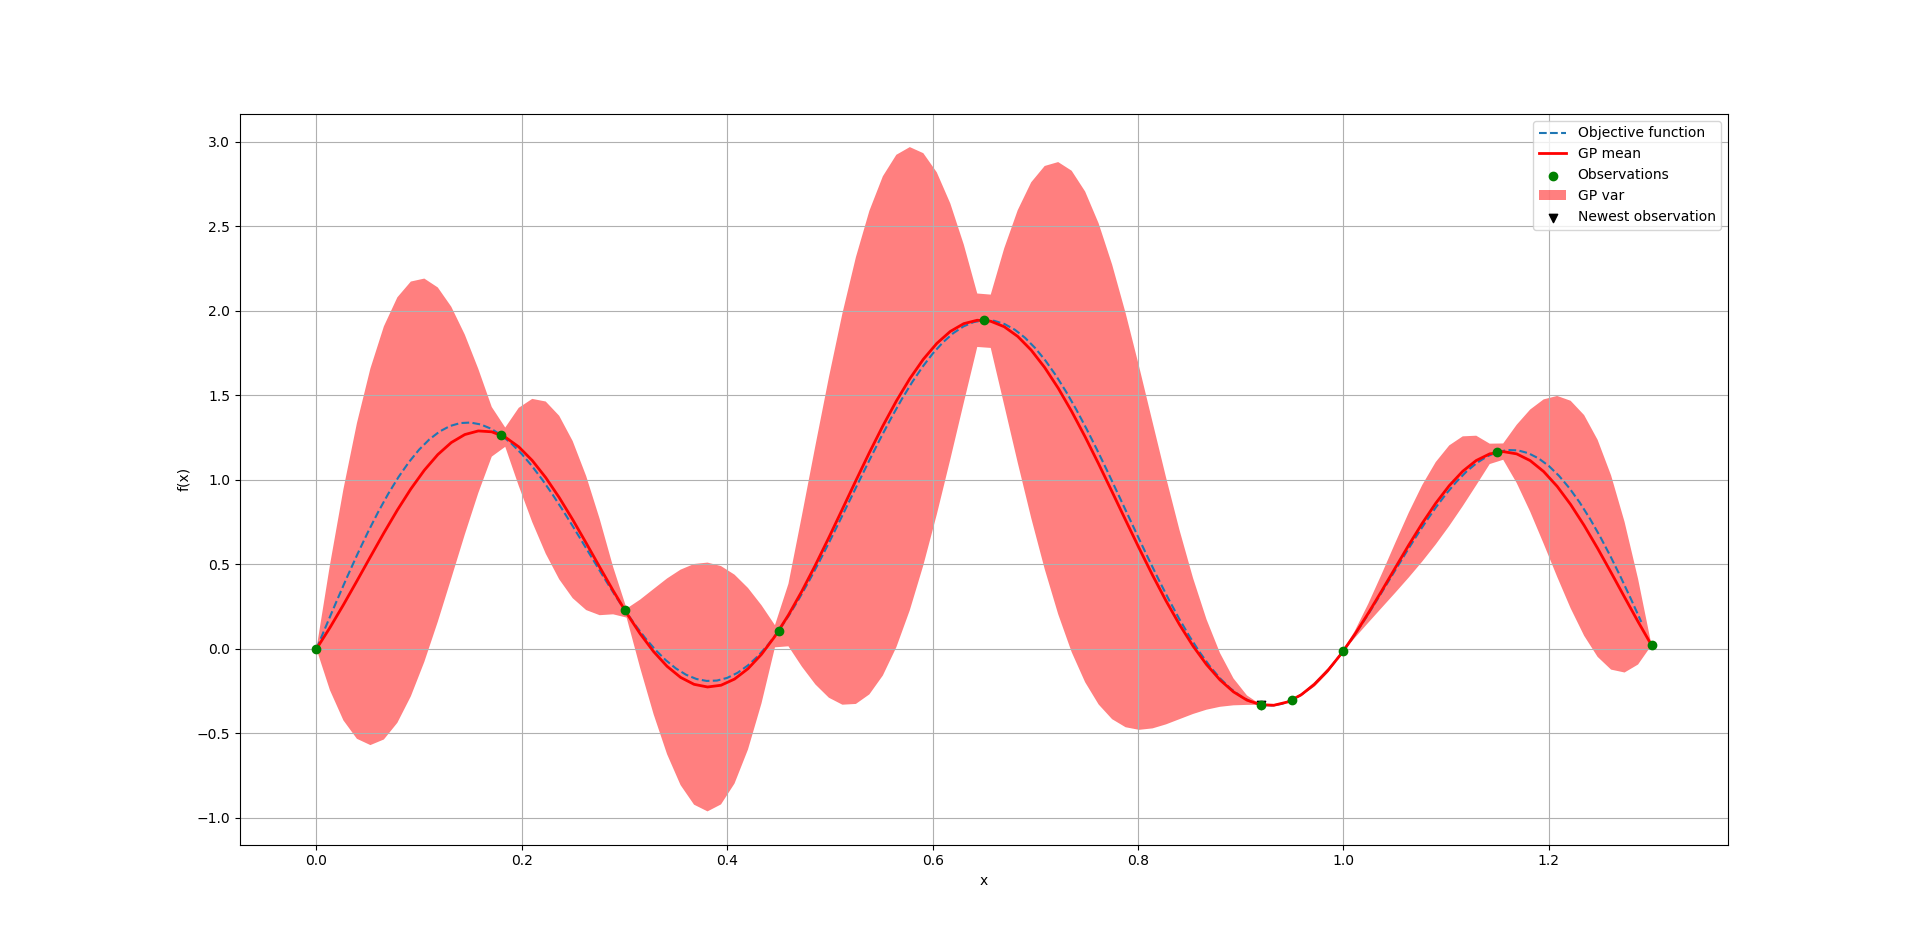
\includegraphics[width=\linewidth]{images/intro_images/BOLoop_8.png}}
%\end{figure}
%\end{frame}
%----------------------------------------------------------------------

\begin{frame}[c]{Bayesian Optimization: Pseudocode}

\begin{center}
\begin{minipage}{0.75\textwidth}
\begin{algorithm}[H]
    %\DontPrintSemicolon
%    \SetAlgoLined
    \setcounter{AlgoLine}{0}
    \SetKwInOut{Require}{Require}
    \SetKwInOut{Result}{Result}
    
    \Require{Search space $\pcs$, 
    		cost function $\cost$, 
    		acquisition function $\acq$, predictive model $\surro$,
    		maximal number of function evaluations $\bobudget$}
    \Result{Best configuration $\finconf$
    (according to $\dataset$ or 
    $\surro$)}
    
	Initialize data $\iter[0]{\dataset}$ with initial observations\;% \leftarrow \varnothing$\; 
	 
    \For{$\bocount=1$ \KwTo $\bobudget$}{
		%\While{$B$ not exhausted} {
		Fit predictive model $\iter[\bocount]{\surro}$ on $\iter[\bocount-1]{\dataset}$\;
		
		Select next query point: $\bonextsample \in \argmax_{\conf \in \pcs} \acq(\conf; \iter[\bocount-1]{\dataset}, \iter[\bocount]{\surro})$\;
		
		Query $\bonextobs$\;
		
		Update data: $\iter[\bocount]{\dataset} \leftarrow \iter[\bocount-1]{\dataset} \cup \{\langle \bonextsample, \bonextobs \rangle \}$\;
	}
	\caption*{BO loop}
\end{algorithm}
\end{minipage}
\end{center}
\end{frame}
%-----------------------------------------------------------------------
\begin{frame}[c]{Bayesian Optimization: Origin of the Name}

\begin{itemize}
    \item Bayesian optimization uses \alert{Bayes' theorem}: 
    	\begin{equation*}
    	    P(A \vert B) = \frac{P(B \vert A) \times  P(A)}{P(B)}
    	    \propto P(B \vert A) \times  P(A)
    	\end{equation*} 
    \item Bayesian optimization uses this to compute a posterior over functions: 
        \begin{equation*}
            P(\func \vert \dataset_{1:\bocount}) \propto P(\dataset_{1:\bocount} \vert \func) \times P(\func), \text{~~~~ where } \dataset_{1:\bocount} = \left \{ \conf_{1:\bocount}, \cost(\conf_{1:\bocount}) \right\}
        \end{equation*} 
\pause
\vspace*{-0.5cm}
    \item Meaning of the individual terms:
        \begin{itemize}
            \item $P(f)$ is the \alert{prior} over functions, which represents our belief about the space of possible objective functions \alert{before} we see any data
            \item $\dataset_{1:\bocount}$ is the \alert{data} (or observations, evidence)
            \item $P(\dataset_{1:\bocount} \vert \func)$ is the likelihood of the data given a function
            \item $P(\func \vert \dataset_{1:\bocount})$ is the \alert{posterior} probability over functions given the data
        \end{itemize}
    \end{itemize}
\end{frame}
%-----------------------------------------------------------------------
\begin{frame}[c]{Bayesian Optimization: Advantages and Disadvantages}

\begin{columns}[T] % align columns
\begin{column}{.48\textwidth}


\begin{block}{Advantages}
\begin{itemize}
  \item Sample efficient 
  \item Can handle noise
  \item Native incorporation of priors 
  \item Does not require gradients 
  \item Theoretical guarantees
\end{itemize}
\end{block}

\end{column}%

\hfill%
\pause 
\begin{column}{.48\textwidth}

\begin{block}{Disadvantages}
\begin{itemize}
  \item Overhead because of model training in each iteration 
  \item Crucially relies on robust surrogate model
%  \item Inherently sequential (in its basic form)
\end{itemize}
\end{block}

\end{column}
\end{columns}

\end{frame}

%-----------------------------------------------------------------------
\begin{frame}[c]{Questions to Answer for Yourself / Discuss with Friends}

\begin{itemize}
    \item \alert{Repetition.} What is Bayesian about Bayesian optimization?
\medskip
    \item \alert{Repetition.} Write down the steps of the BO loop.
\medskip
    \item \alert{Discussion.} Can you think of an expensive blackbox optimization problem other than hyperparameter optimization?
\end{itemize}

\end{frame}

%-----------------------------------------------------------------------
\begin{frame}[c]{Learning Goals of this Lecture}
\framesubtitle{After this lecture, students can ...}

\begin{itemize}
    \item Explain the basics of Bayesian optimization
    \item Derive \alert{simple acquisition functions}
    \item Describe \alert{complex lookahead acquisition functions}
    \item Describe possible \alert{surrogate models} and their pros and cons 
    \item Discuss the \alert{limits of Bayesian optimization} and extensions to tackle these
%    \item Describe the \alert{alternative Bayesian optimization approach of TPE}
    \item Discuss \alert{success stories} of Bayesian optimization
\end{itemize}

\end{frame}

%-----------------------------------------------------------------------
%----------------------------------------------------------------------
%\begin{frame}[c]{Surrogate modelling}
%\framesubtitle{General idea}
%\begin{itemize}
%    \item Use a surrogate model of the expensive function $\cost$ as a cheap-to-evaluate proxy.
%    \begin{itemize}
%        \item Use a probabilistic model with well-calibrated uncertainty predictions.
%    \end{itemize}
%    \fhpause
%    \item Define a utility function to guide the search for new data points.
%    \fhpause
%    \item Use the optimization of the utility function as a decision procedure to provide inference on where to evaluate next.
%
%\end{itemize}
%\end{frame}

%-----------------------------------------------------------------------

\end{document}